\section{Feature Set and Functional Capabilities}
\label{sec:feature-set}

This section presents a comprehensive description of the system's feature set, organized by functional domain and implementation complexity. Our current prototype\footnote{The current prototype version of the AMEO Analytics scheduling software was developed to demonstrate capability only. A full production version requires a rigorous software-quality assessment and thorough testing and integration of several additional capabilites to ensure security and compatibility with Tennislink softawre.} already contains draft versions of the features identified in Section~I of the RFP. Table~\ref{tab:rfp-compliance} provides a comprehensive mapping of the required features specified in the RFP Services Overview to the current prototype implementation status and relevant documentation sections. 

\begin{table}[htbp]
\centering
\caption{Implementation Status of Required RFP Features: Current Prototype Capabilities and Planned Development Timeline }
\label{tab:rfp-compliance}
\small
\begin{tabular}{|p{0.7\textwidth}|p{0.25\textwidth}|}
\hline
\textbf{Required Feature} & \textbf{Current Status} \\
\hline
Venue and Court Availability Management & In Prototype \\
\hline
UI for facilities/admins to enter availability & In Prototype \\
\hline
Ability to ingest team matchups from Tennislink & Phase 1 and 2 \\
\hline
Blackout dates & In Prototype \\
\hline
Match Generation with Home/away balance & In Prototype \\
\hline
Scheduling with Split start times & In Prototype \\
\hline
Facility management & In Prototype \\
\hline
Scheduling Conflict Avoidance & In Prototype \\
\hline
Match deletion/editing & In Prototype \\
\hline
Write schedule back to Tennislink & Phase 1 and 2 \\
\hline
\end{tabular}
\end{table}


\subsection{Core Application Infrastructure}

\subsubsection{Administrative Dashboard and System Navigation}
The system provides a centralized administrative interface designed to facilitate efficient operation management and system oversight:



\begin{itemize}
    \item \textbf{Unified Navigation Architecture}: Implements intuitive access pathways to all major functional modules (Facilities, Leagues, Teams, Matches) through a hierarchical menu system
    \item \textbf{Import/Export}: Comprehensive YAML and JSON data interchange functionality with structured schema validation and bulk operations support for leagues, facilities, teams, and match data 
    \item \textbf{System Health Monitoring}: Continuous monitoring of database connectivity, system performance indicators, and operational health metrics
    \item \textbf{Administrative Workflows}: Streamlined access to frequently executed operations including automated match generation and intelligent scheduling procedures
    \item \textbf{Responsive User Interface}: Modern Bootstrap-based interface architecture ensuring cross-platform compatibility and quality user experience
\end{itemize}

\begin{figure}[htbp]
\centering
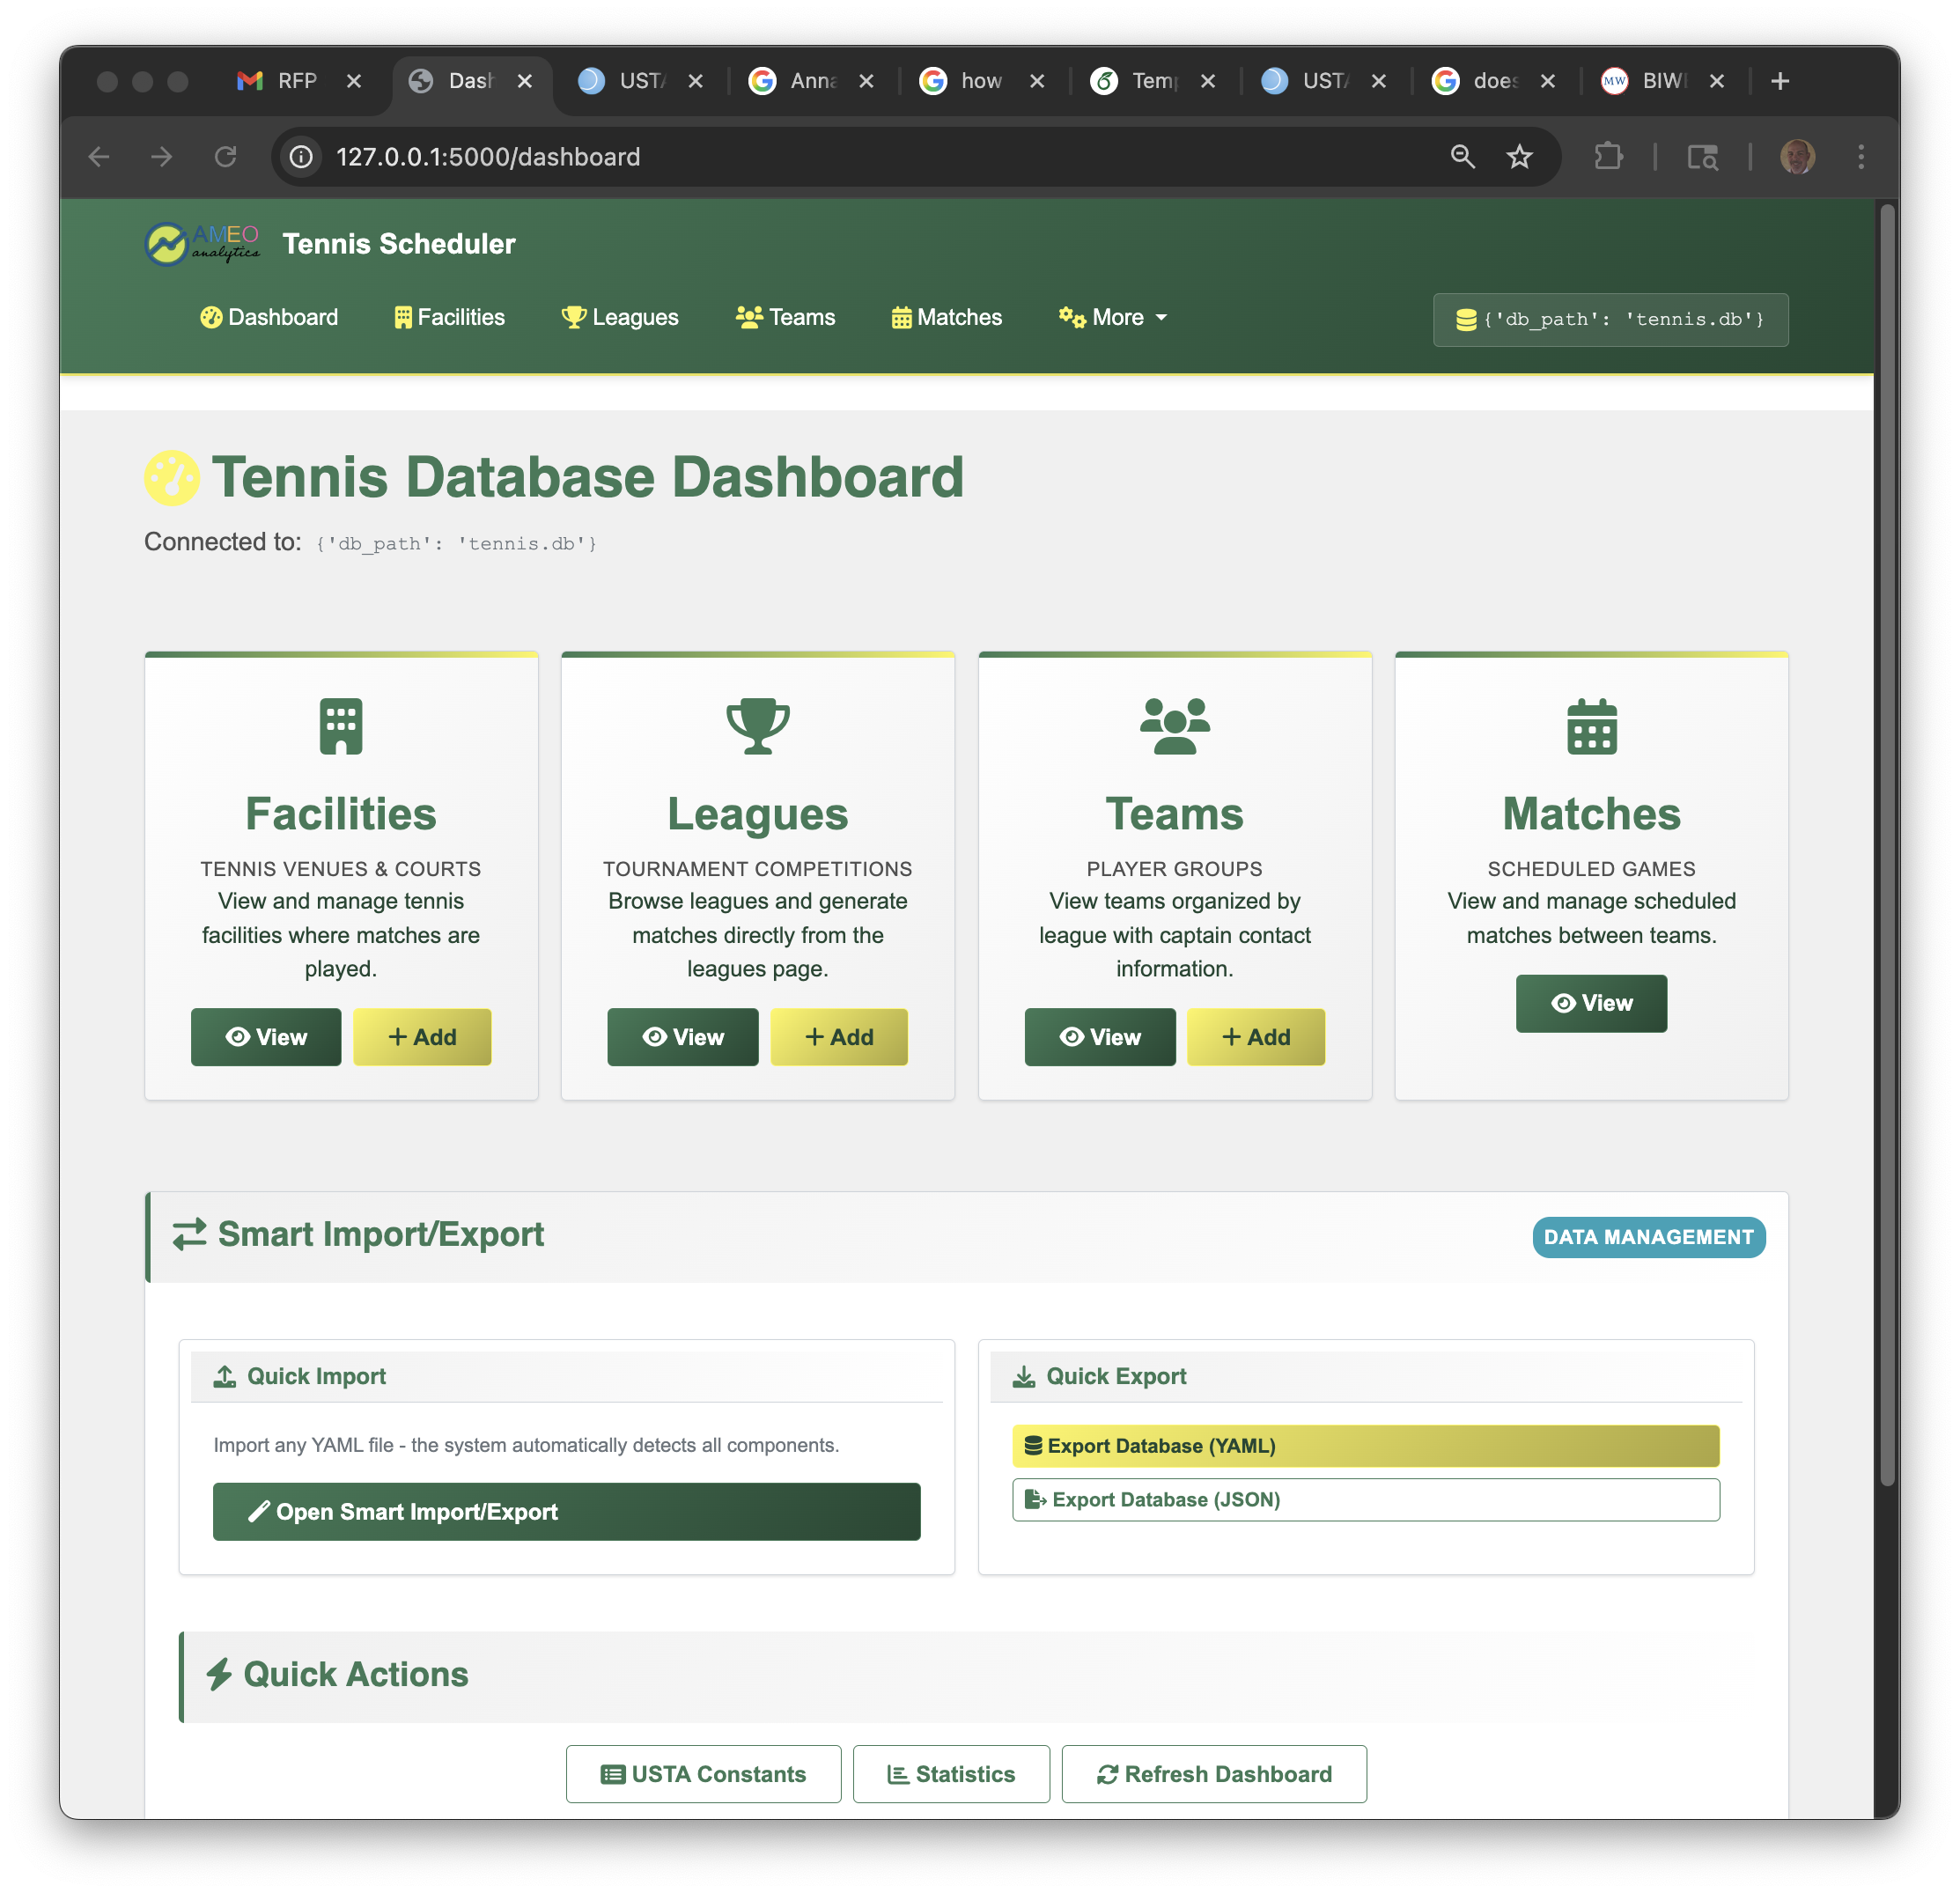
\includegraphics[width=0.6\textwidth]{images/dashboard.png}
\caption{Administrative Dashboard Interface}
\label{fig:dashboard}
\end{figure}

\subsubsection{Facility Resource Management}
\label{sec:facility-management}
The system implements comprehensive facility management capabilities designed to optimize resource allocation and operational efficiency:

\begin{itemize}
    \item \textbf{Facility Information Repository}: Maintains detailed facility profiles including nomenclature, geographical coordinates, court inventory, and operational schedules
    \item \textbf{Advanced Scheduling Infrastructure}: Supports complex temporal availability patterns including weekly recurring schedules, exceptional blackout periods, and court-specific operational constraints
    \item \textbf{Resource Capacity Optimization}: Implements real-time tracking of court availability and temporal slot allocation for enhanced scheduling efficiency
    \item \textbf{Performance Analytics}: Provides comprehensive facility utilization metrics including court occupancy rates, usage distribution analysis, and operational efficiency indicators
    \item \textbf{Administrative Interface}: Features advanced form-based management tools for configuring weekly operational schedules and temporal availability restrictions
    \item \textbf{Data Organization Tools}: Implements multi-criteria sorting capabilities based on facility attributes including nomenclature, location, court capacity, and availability status
\end{itemize}

\begin{figure}[H]
\centering
\begin{minipage}{0.48\textwidth}
\centering
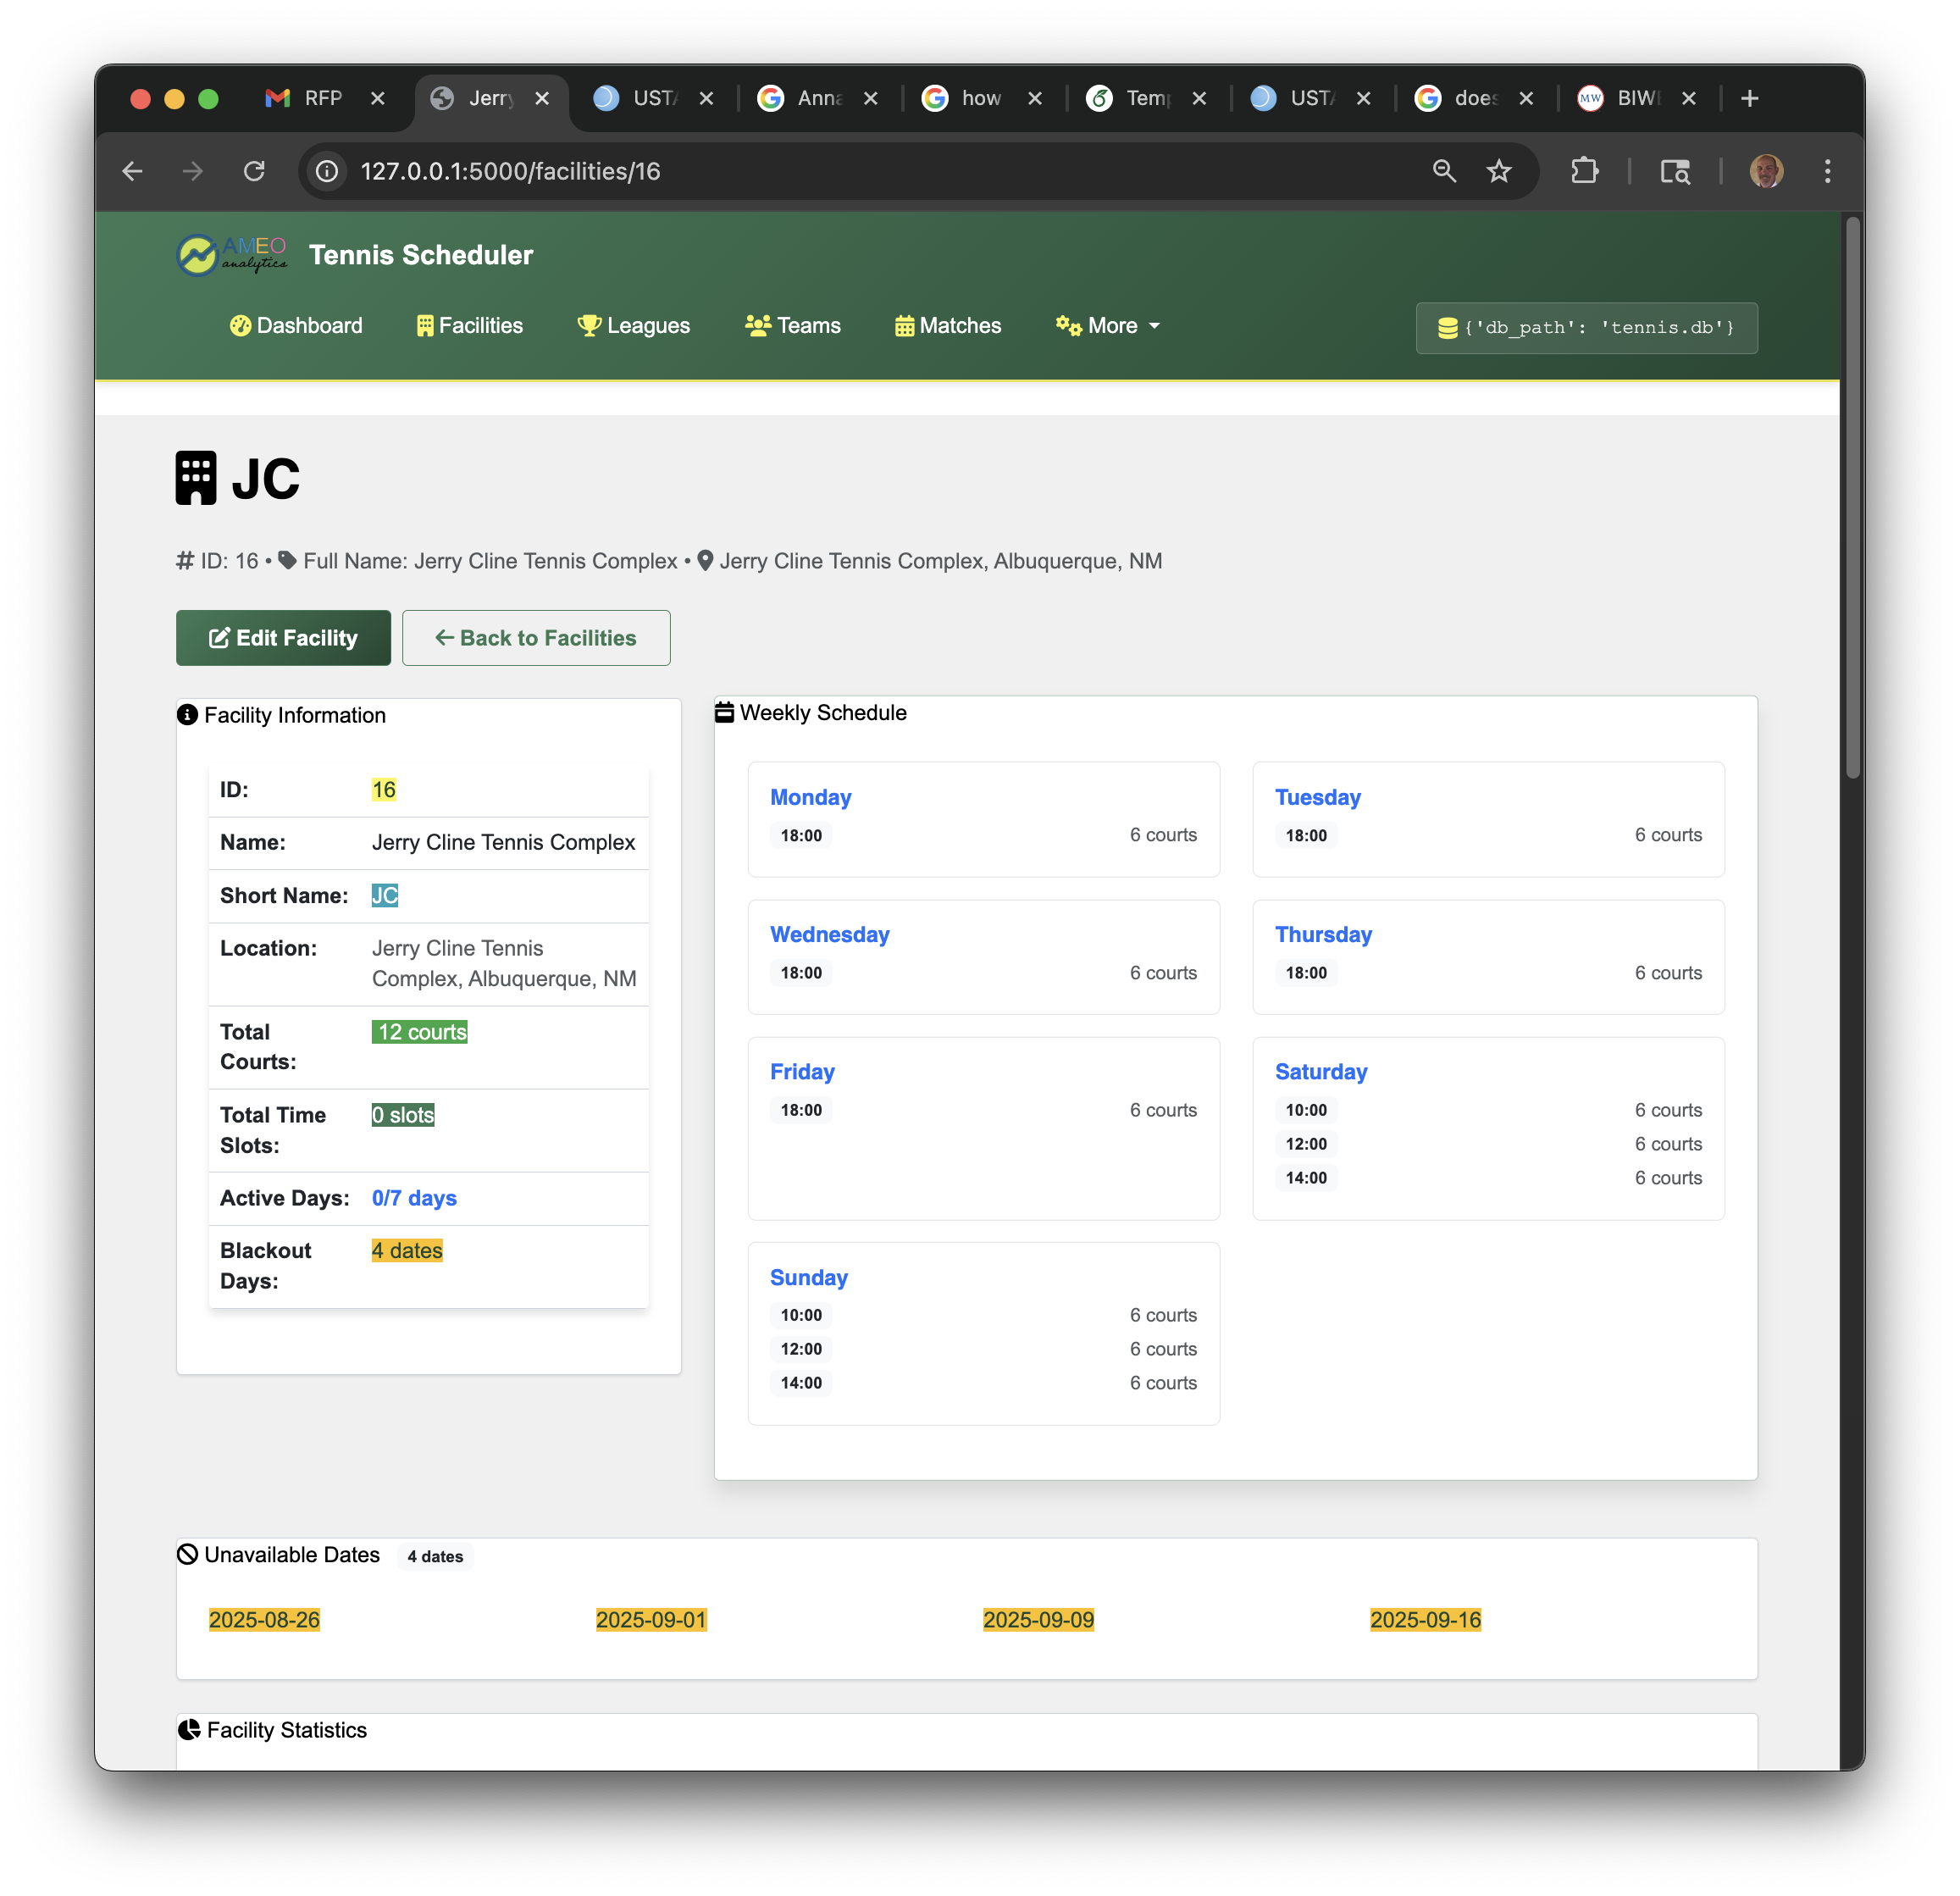
\includegraphics[width=\textwidth]{images/facility-view.png}
\end{minipage}
\hfill
\begin{minipage}{0.48\textwidth}
\centering
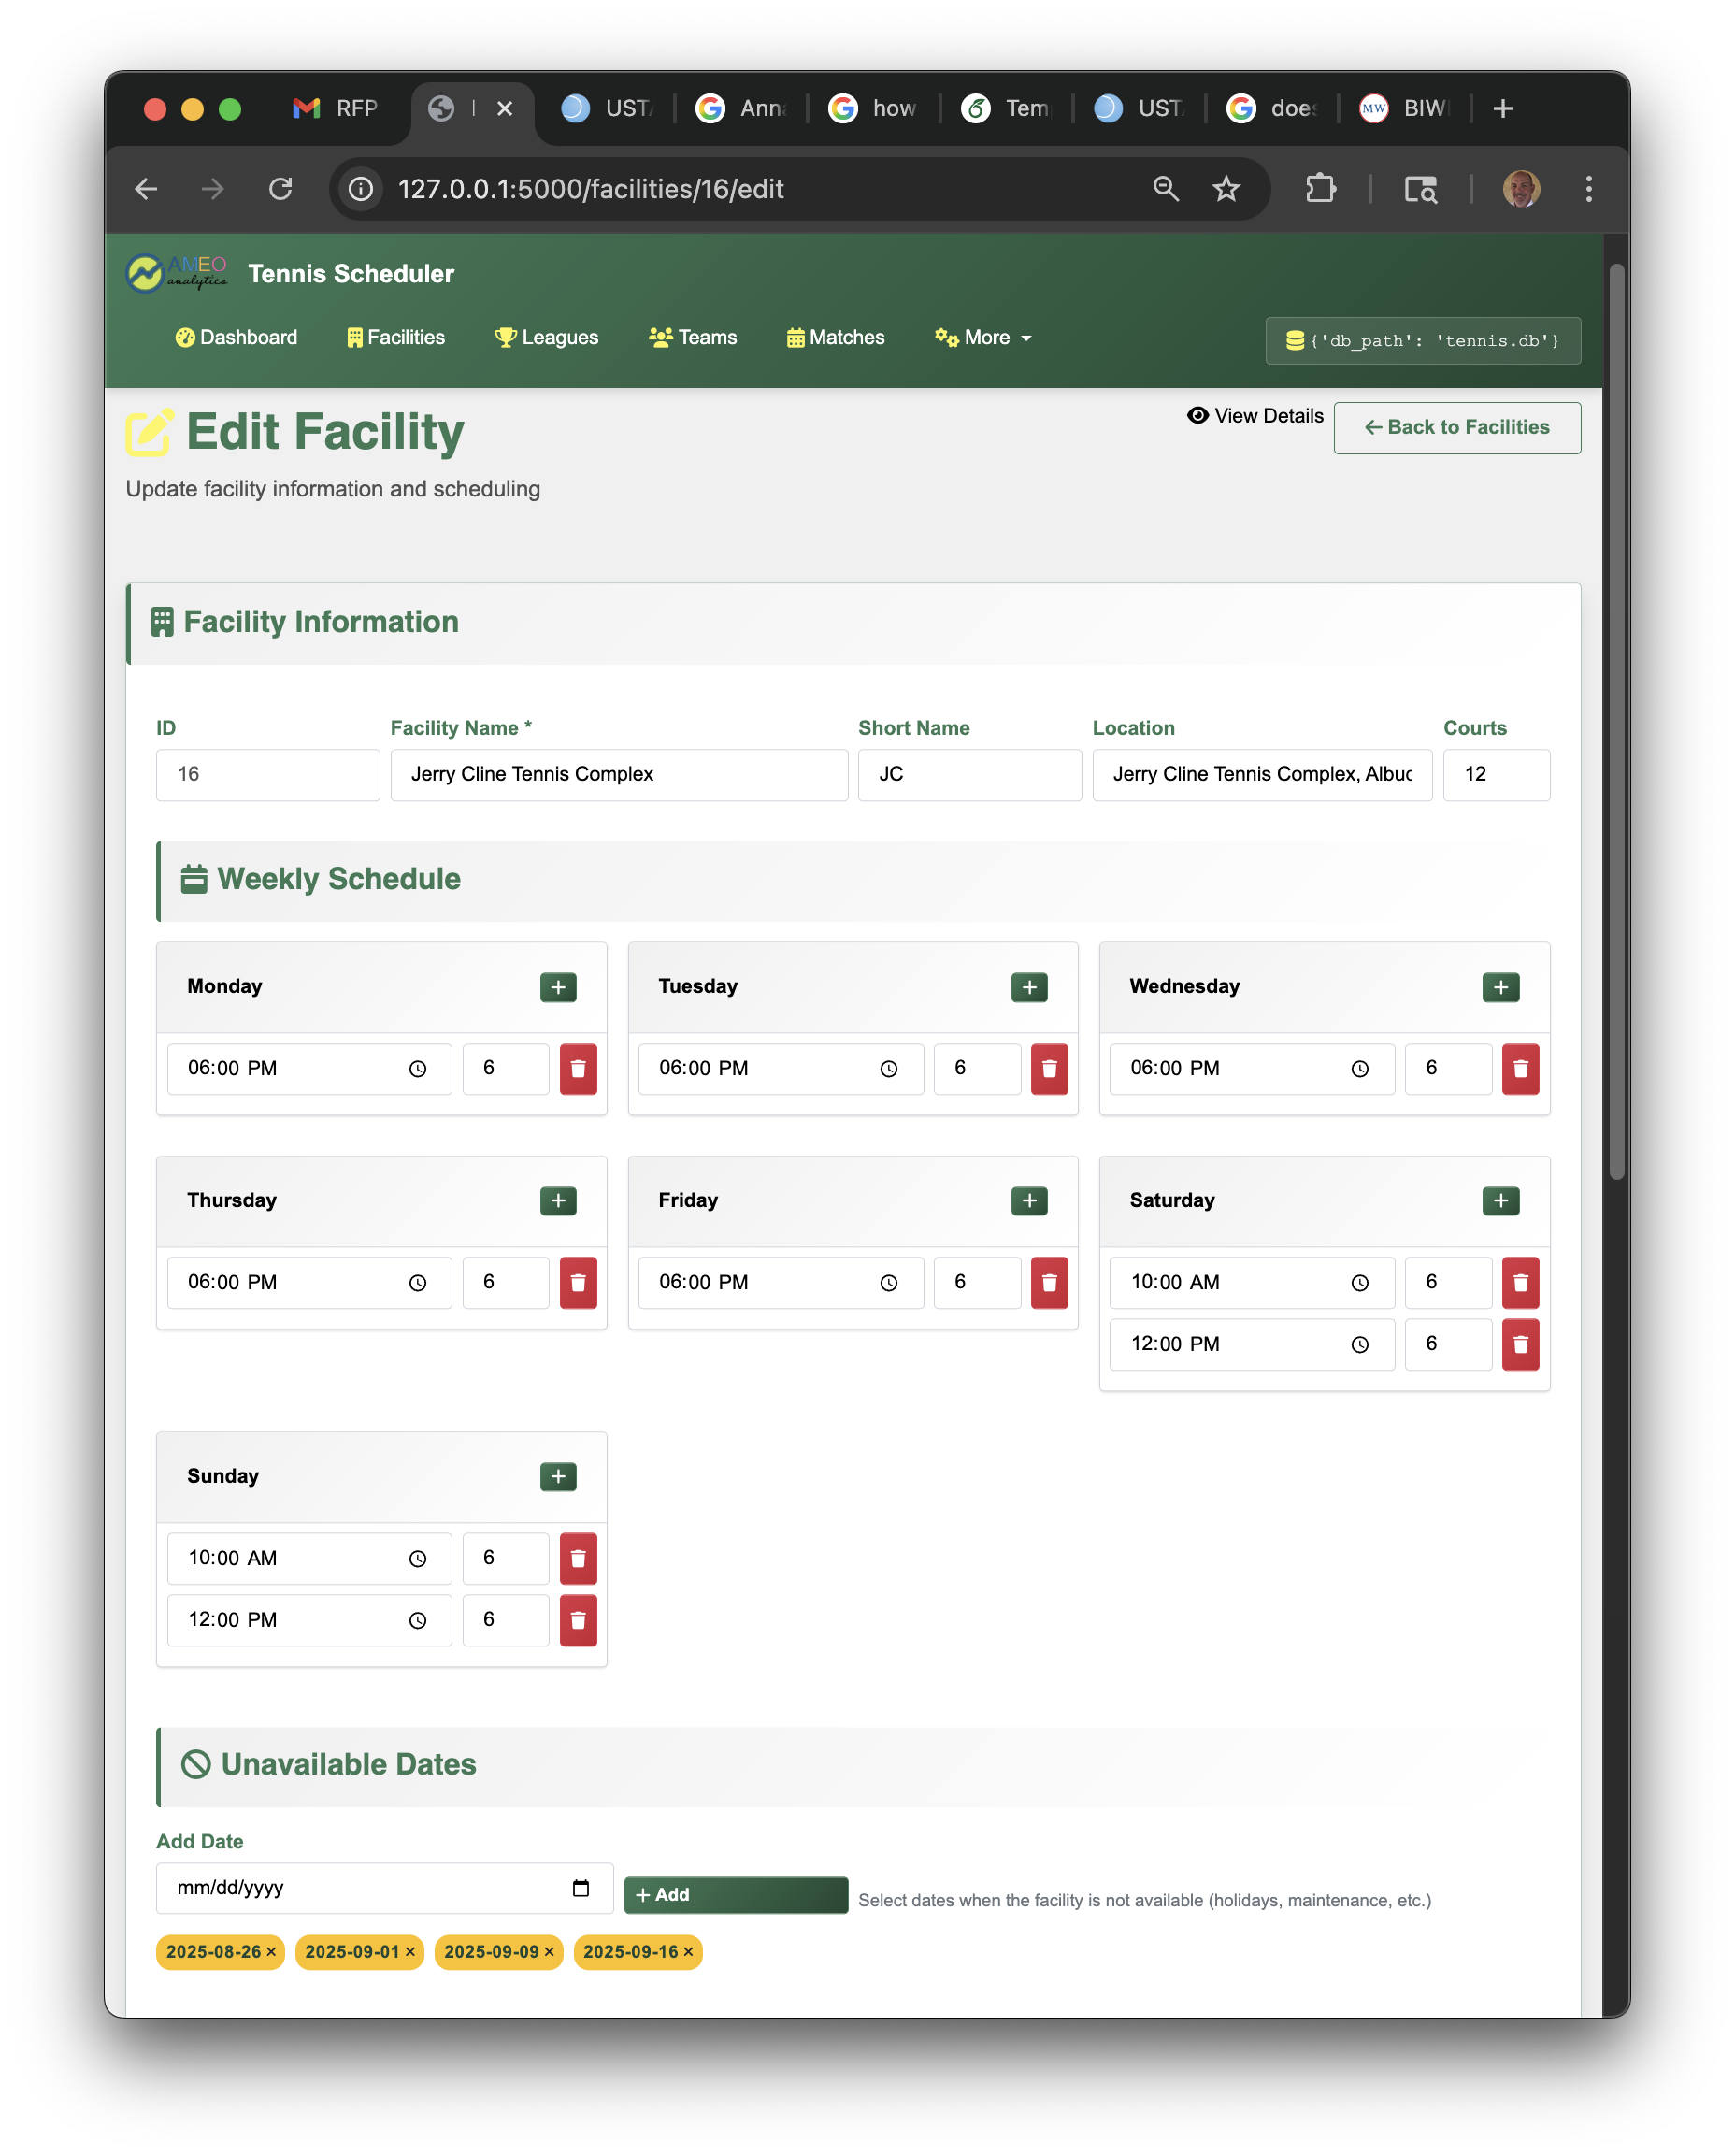
\includegraphics[width=\textwidth]{images/facility-edit.png}
\end{minipage}
\caption{Facility Management Interface: (left) venue details and court information display, (right) facility editing and availability scheduling configuration}
\label{fig:facility-view}
\end{figure}

\subsubsection{League Administration and Governance}
The application provides comprehensive support for league management aligned with USTA organizational standards:

\begin{itemize}
    \item \textbf{USTA Compliance Framework}: Full implementation of official USTA league classification system including year, section, region, age group, and division taxonomies
    \item \textbf{Organizational Scheduling Parameters}: Configurable league-wide scheduling preferences including primary playing days, alternative scheduling periods, and seasonal operational constraints
    \item \textbf{Competition Structure Configuration}: Comprehensive match configuration capabilities including line specifications, tournament format definitions, and temporal round organization
    \item \textbf{Seasonal Operations Management}: Administrative tools for defining season parameters including start/end dates, round scheduling methodology, and league-specific operational rules
    \item \textbf{Team Organizational Framework}: Hierarchical team management within league structures including relationship mapping and scheduling interdependencies
\end{itemize}

\begin{figure}[H]
\centering
\begin{minipage}{0.48\textwidth}
\centering
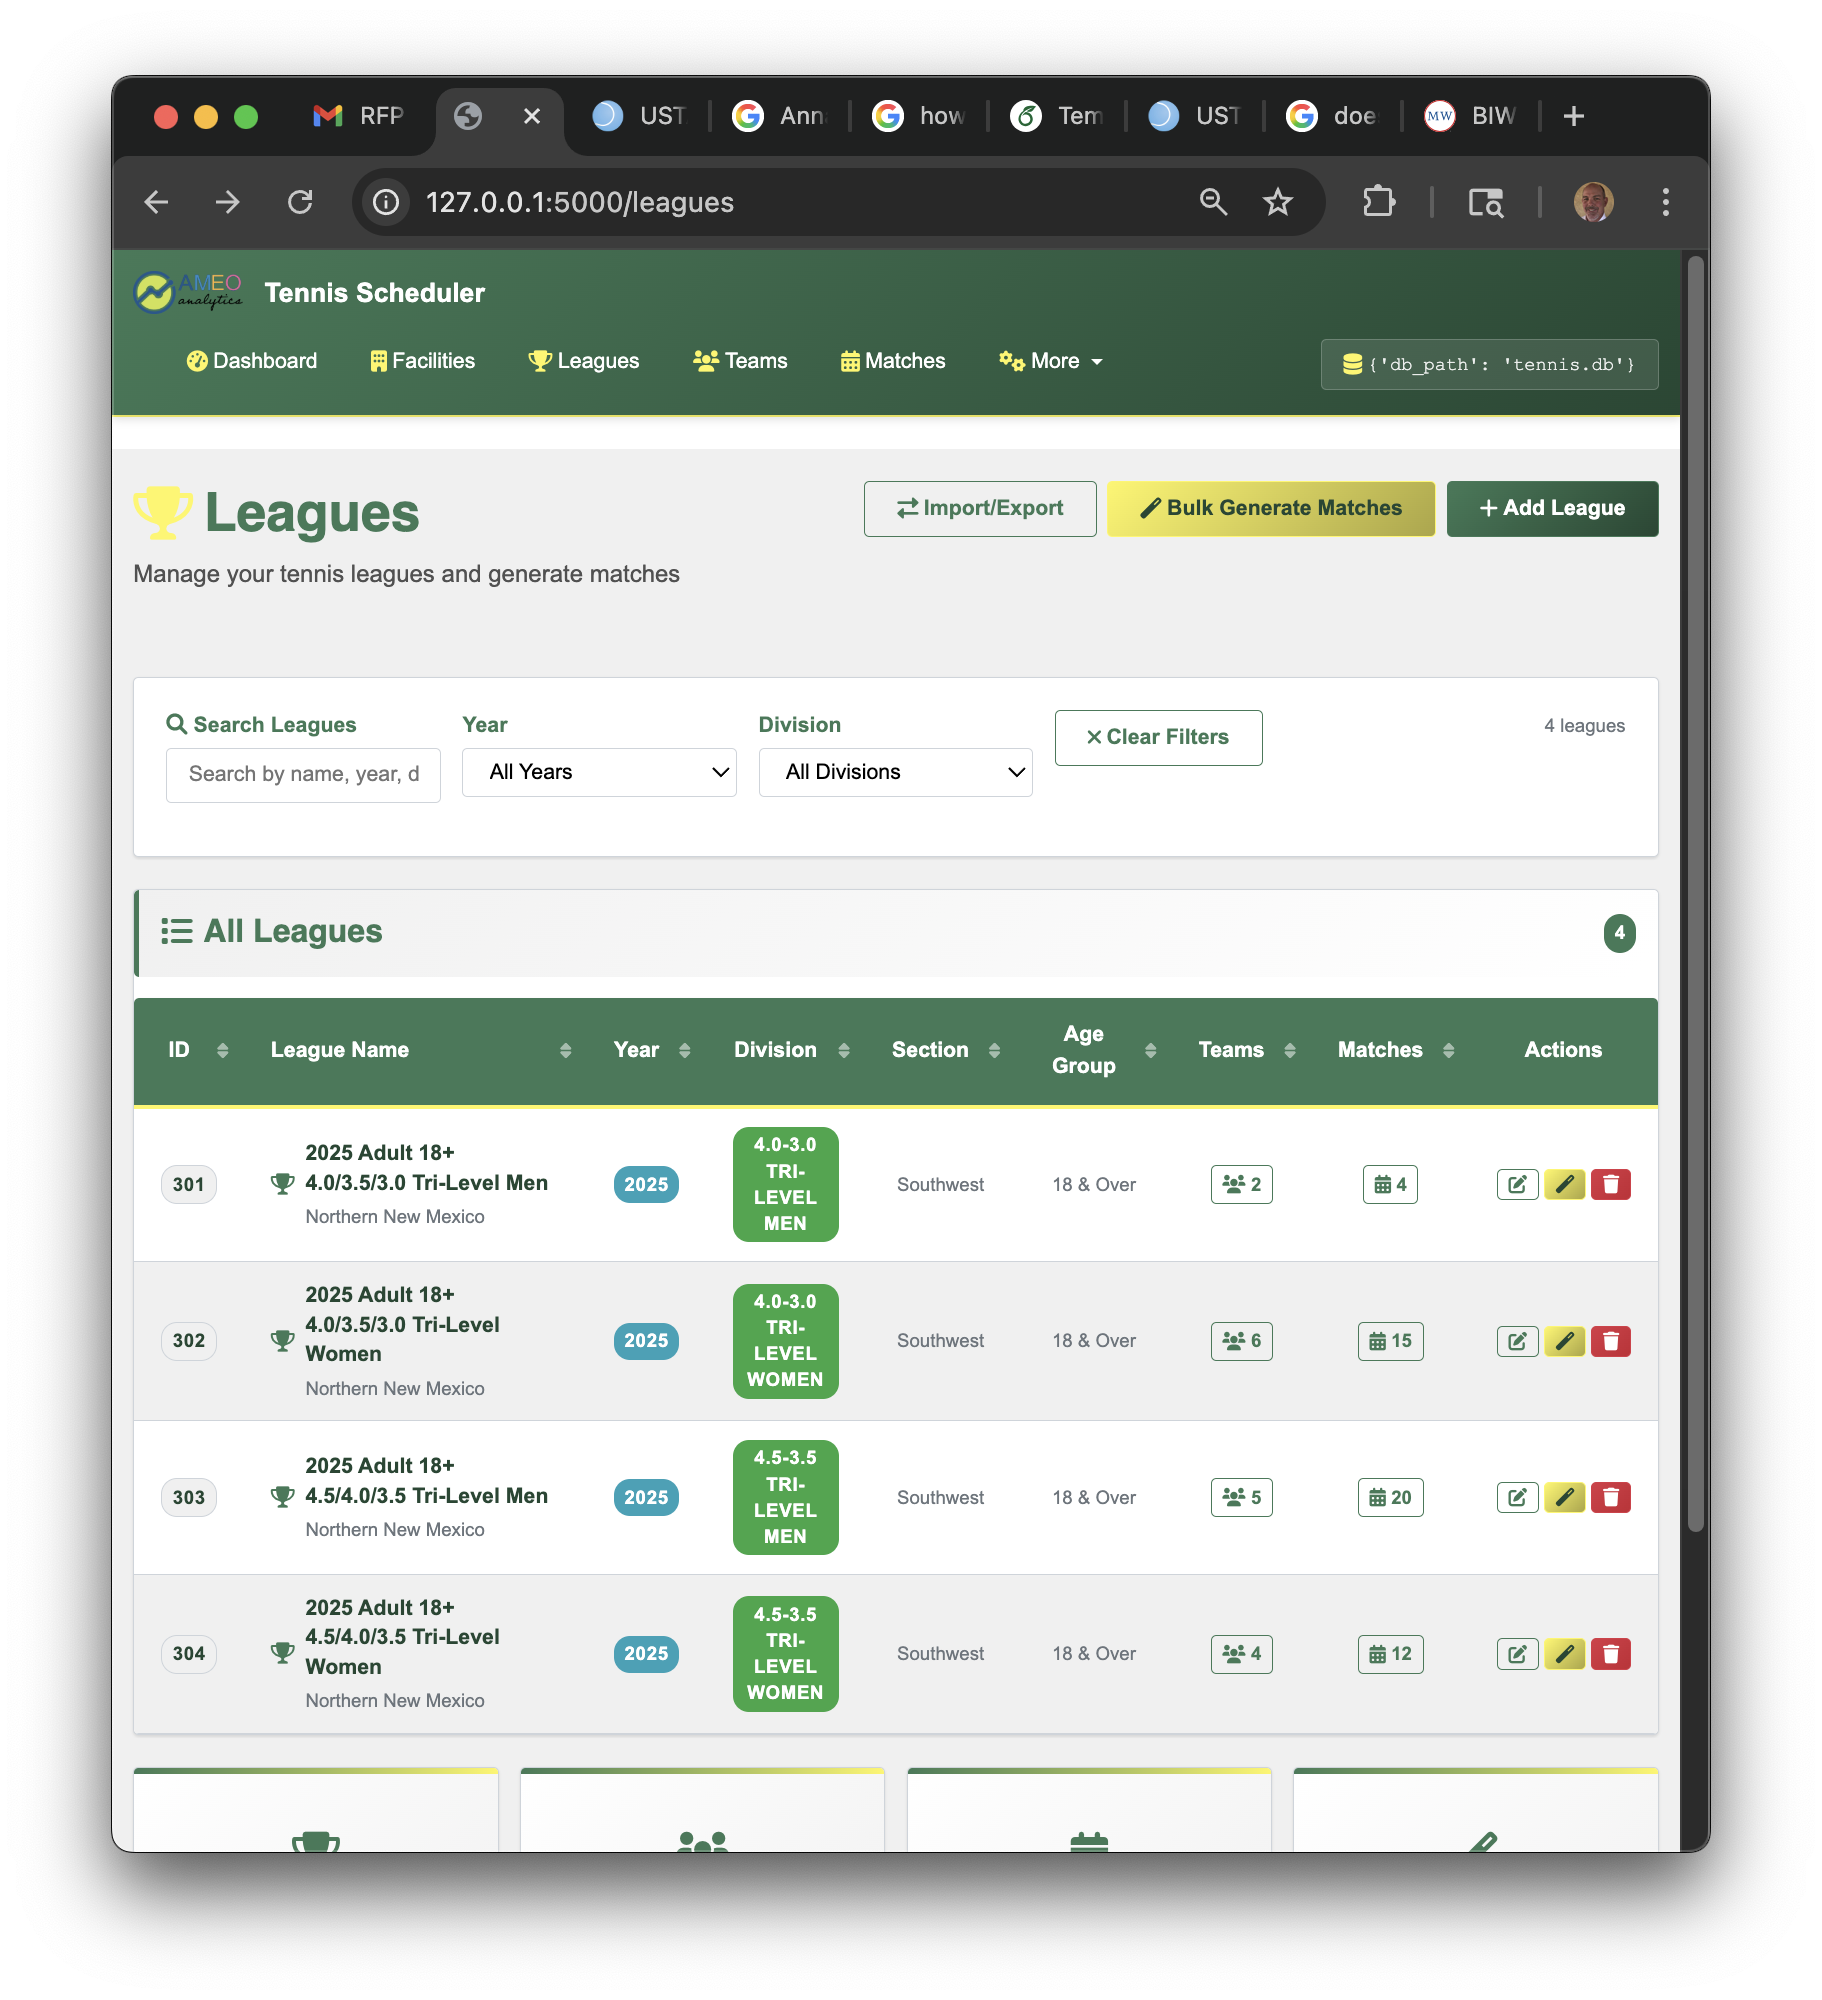
\includegraphics[width=\textwidth]{images/leagues.png}
\end{minipage}
\hfill
\begin{minipage}{0.48\textwidth}
\centering
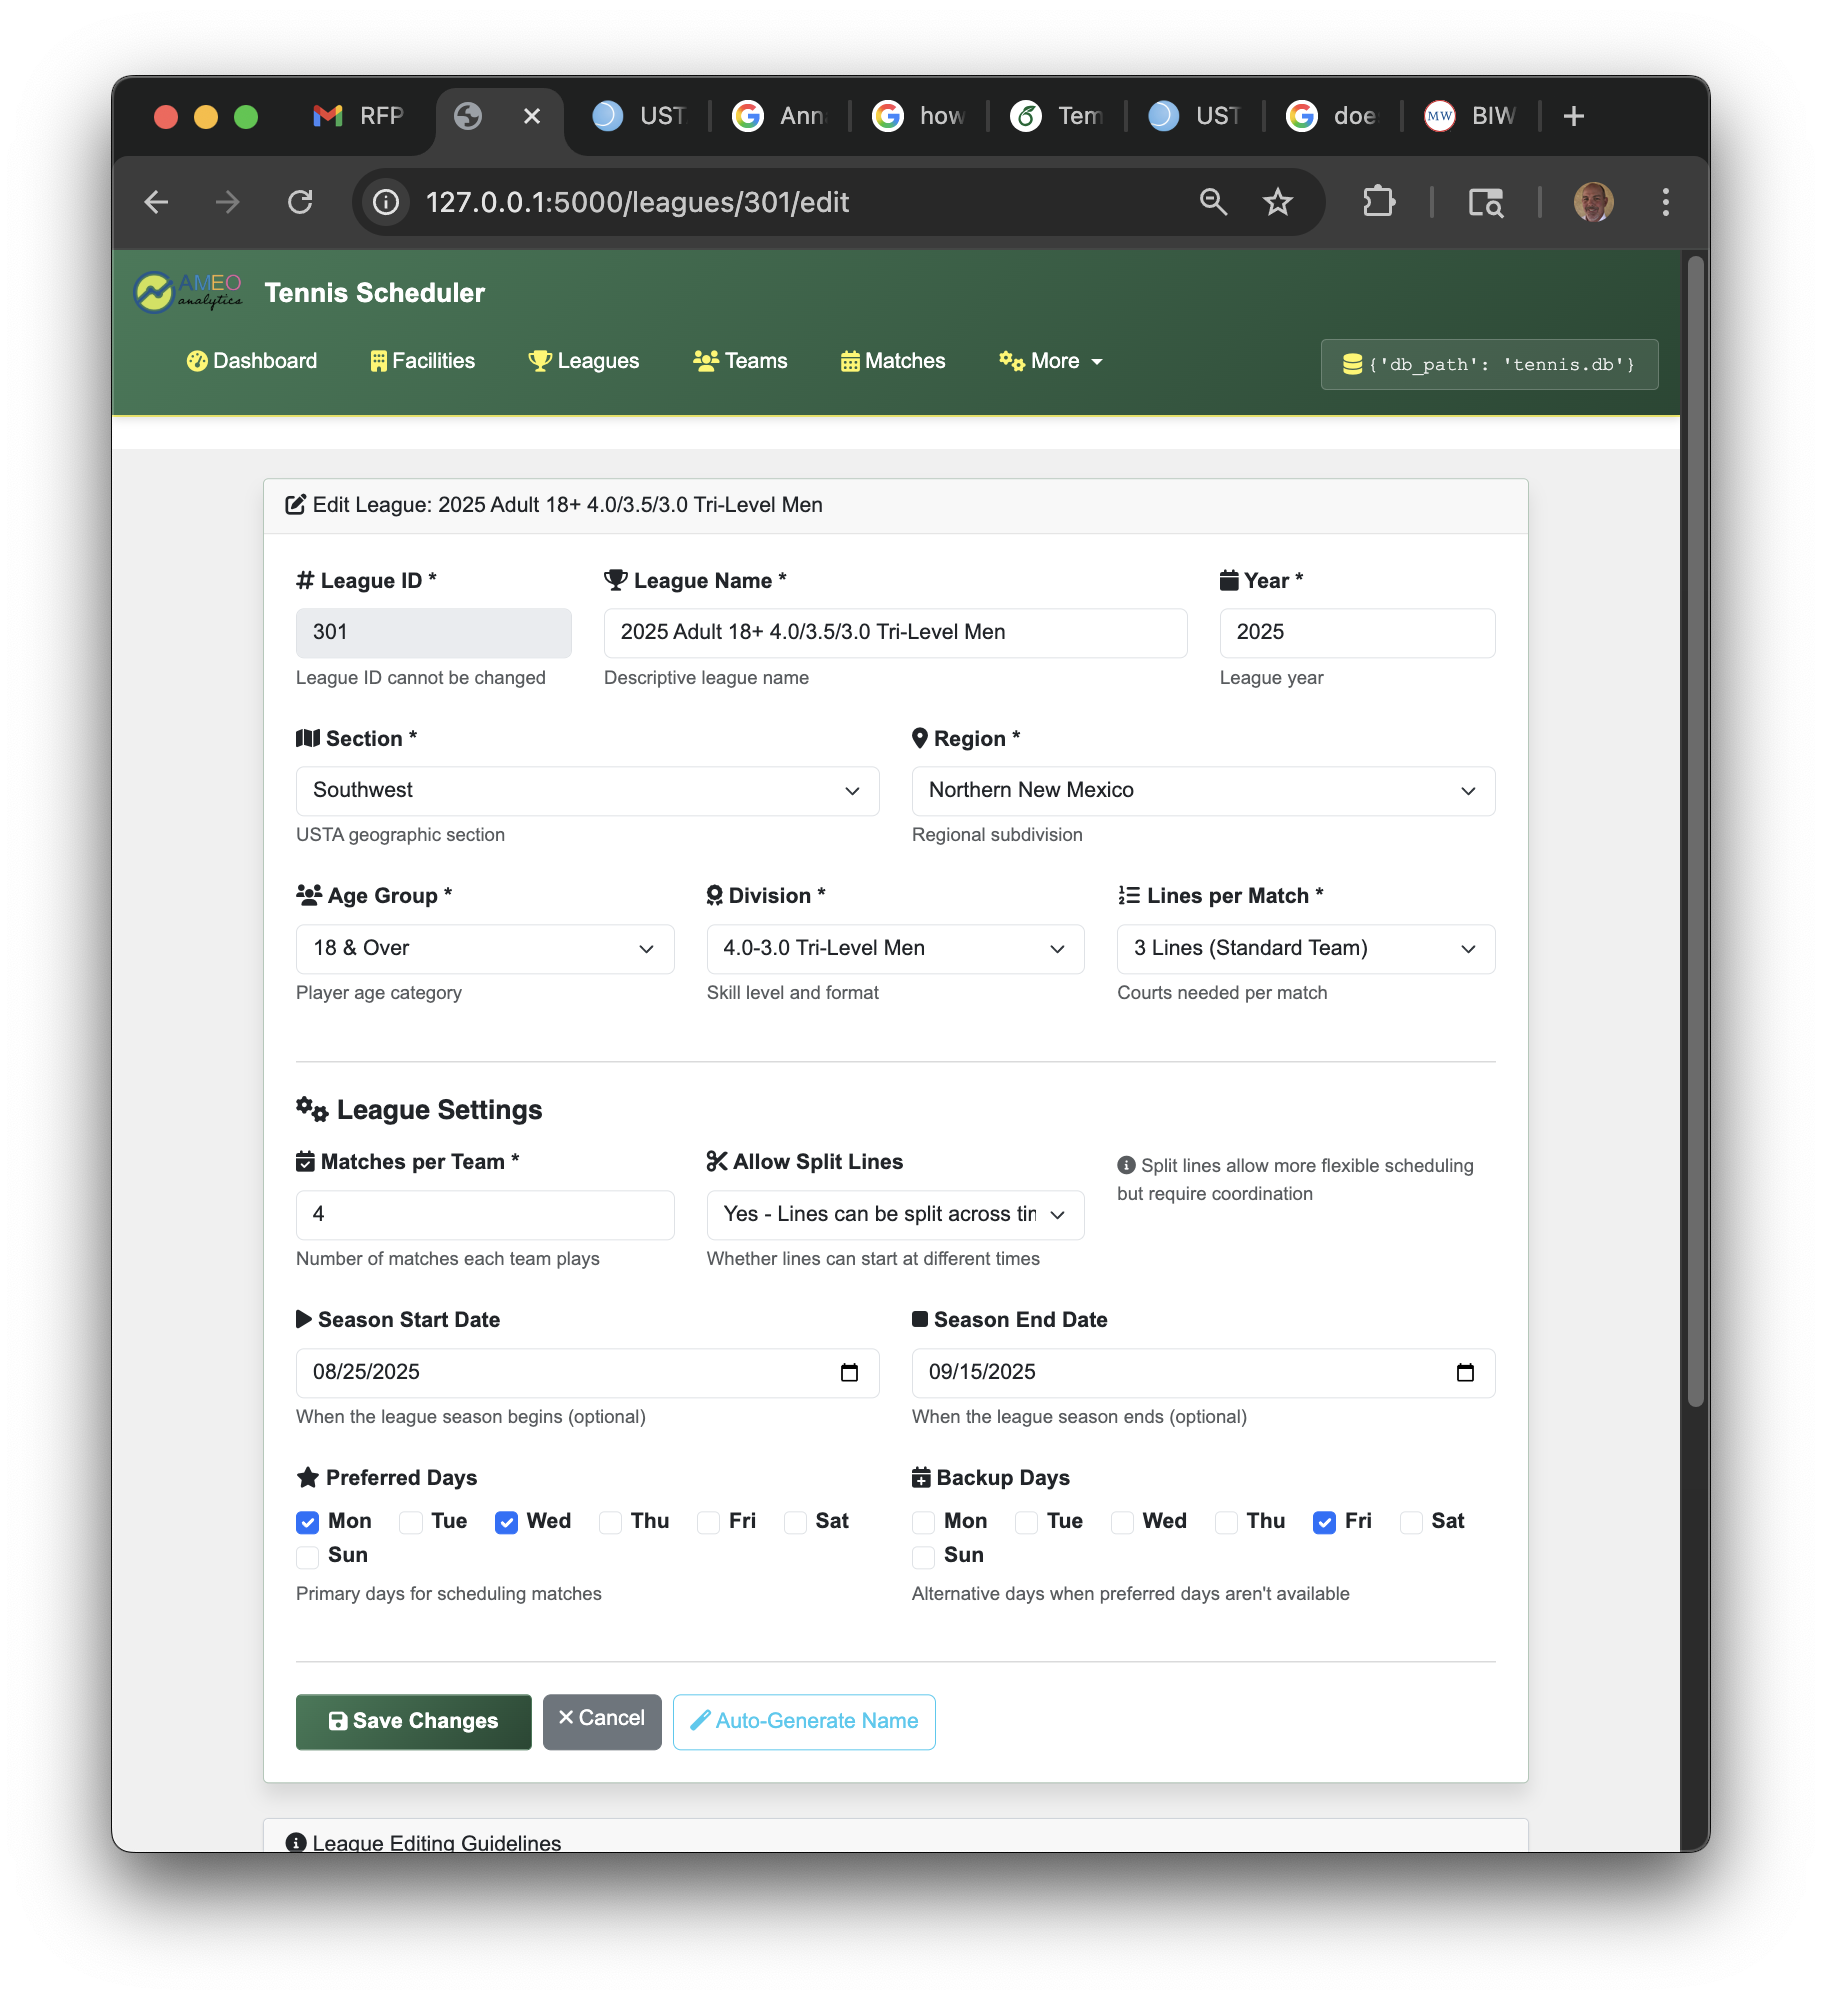
\includegraphics[width=\textwidth]{images/league-edit.png}
\end{minipage}
\caption{League Administration Interface: (left) USTA league listing with organizational structure, (right) league configuration with scheduling parameters and competition structure}
\label{fig:league-administration}
\end{figure}

\subsubsection{Team Management and Coordination}
The system provides sophisticated team management capabilities with enhanced facility coordination:

\begin{itemize}
    \item \textbf{Multi-Facility Assignment Architecture}: Implementation of hierarchical facility preference systems enabling teams to maintain multiple venue associations with priority-based ordering:
    \begin{itemize}
        \item Primary facility designation for initial scheduling optimization
        \item Secondary facility allocations providing scheduling flexibility and conflict resolution
        \item Dynamic priority reordering through intuitive drag-and-drop interface mechanisms
        \item Comprehensive facility management through web-based administrative interfaces
    \end{itemize}
    \item \textbf{Team-Specific Scheduling Preferences}: Configurable temporal preferences including preferred playing days and availability constraint management
    \item \textbf{League Integration Protocols}: Advanced filtering and organizational tools providing detailed league-specific team information and hierarchical relationships
    \item \textbf{Intelligent Facility Selection}: Automated facility selection algorithms considering real-time availability, capacity constraints, and team preference hierarchies
\end{itemize}

\begin{figure}[H]
\centering
\begin{minipage}{0.48\textwidth}
\centering
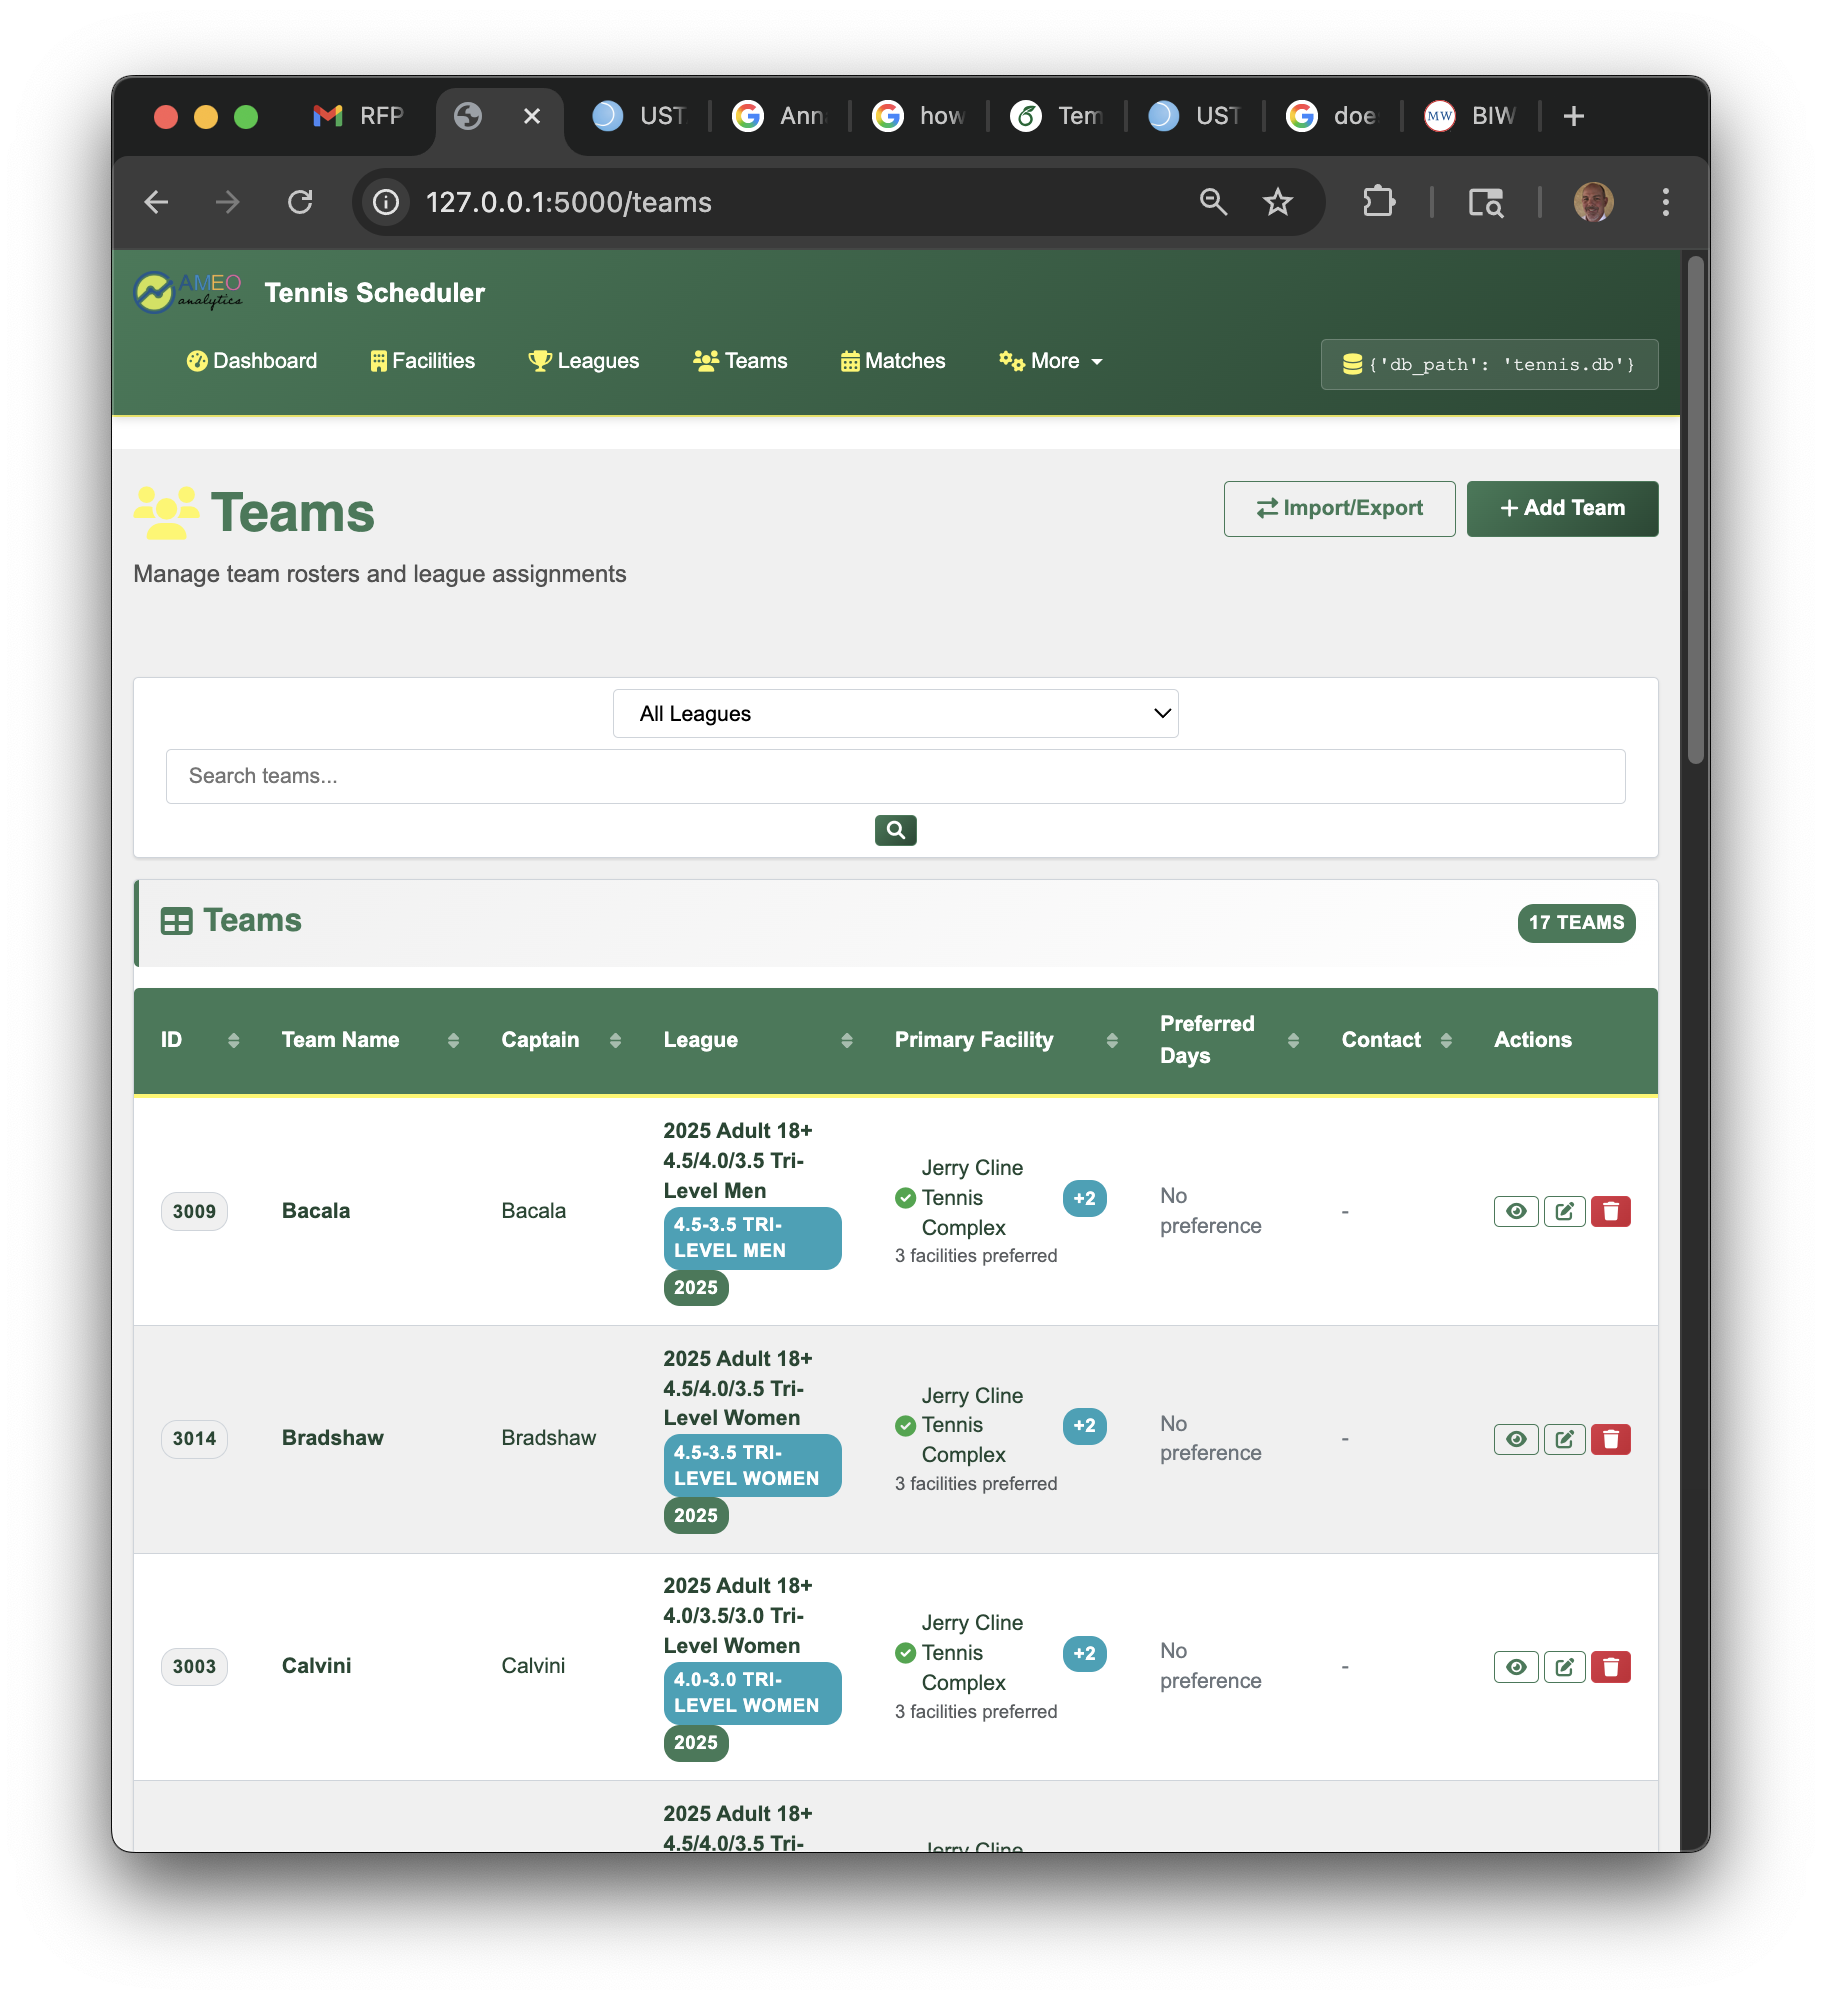
\includegraphics[width=\textwidth]{images/teams.png}
\end{minipage}
\hfill
\begin{minipage}{0.48\textwidth}
\centering
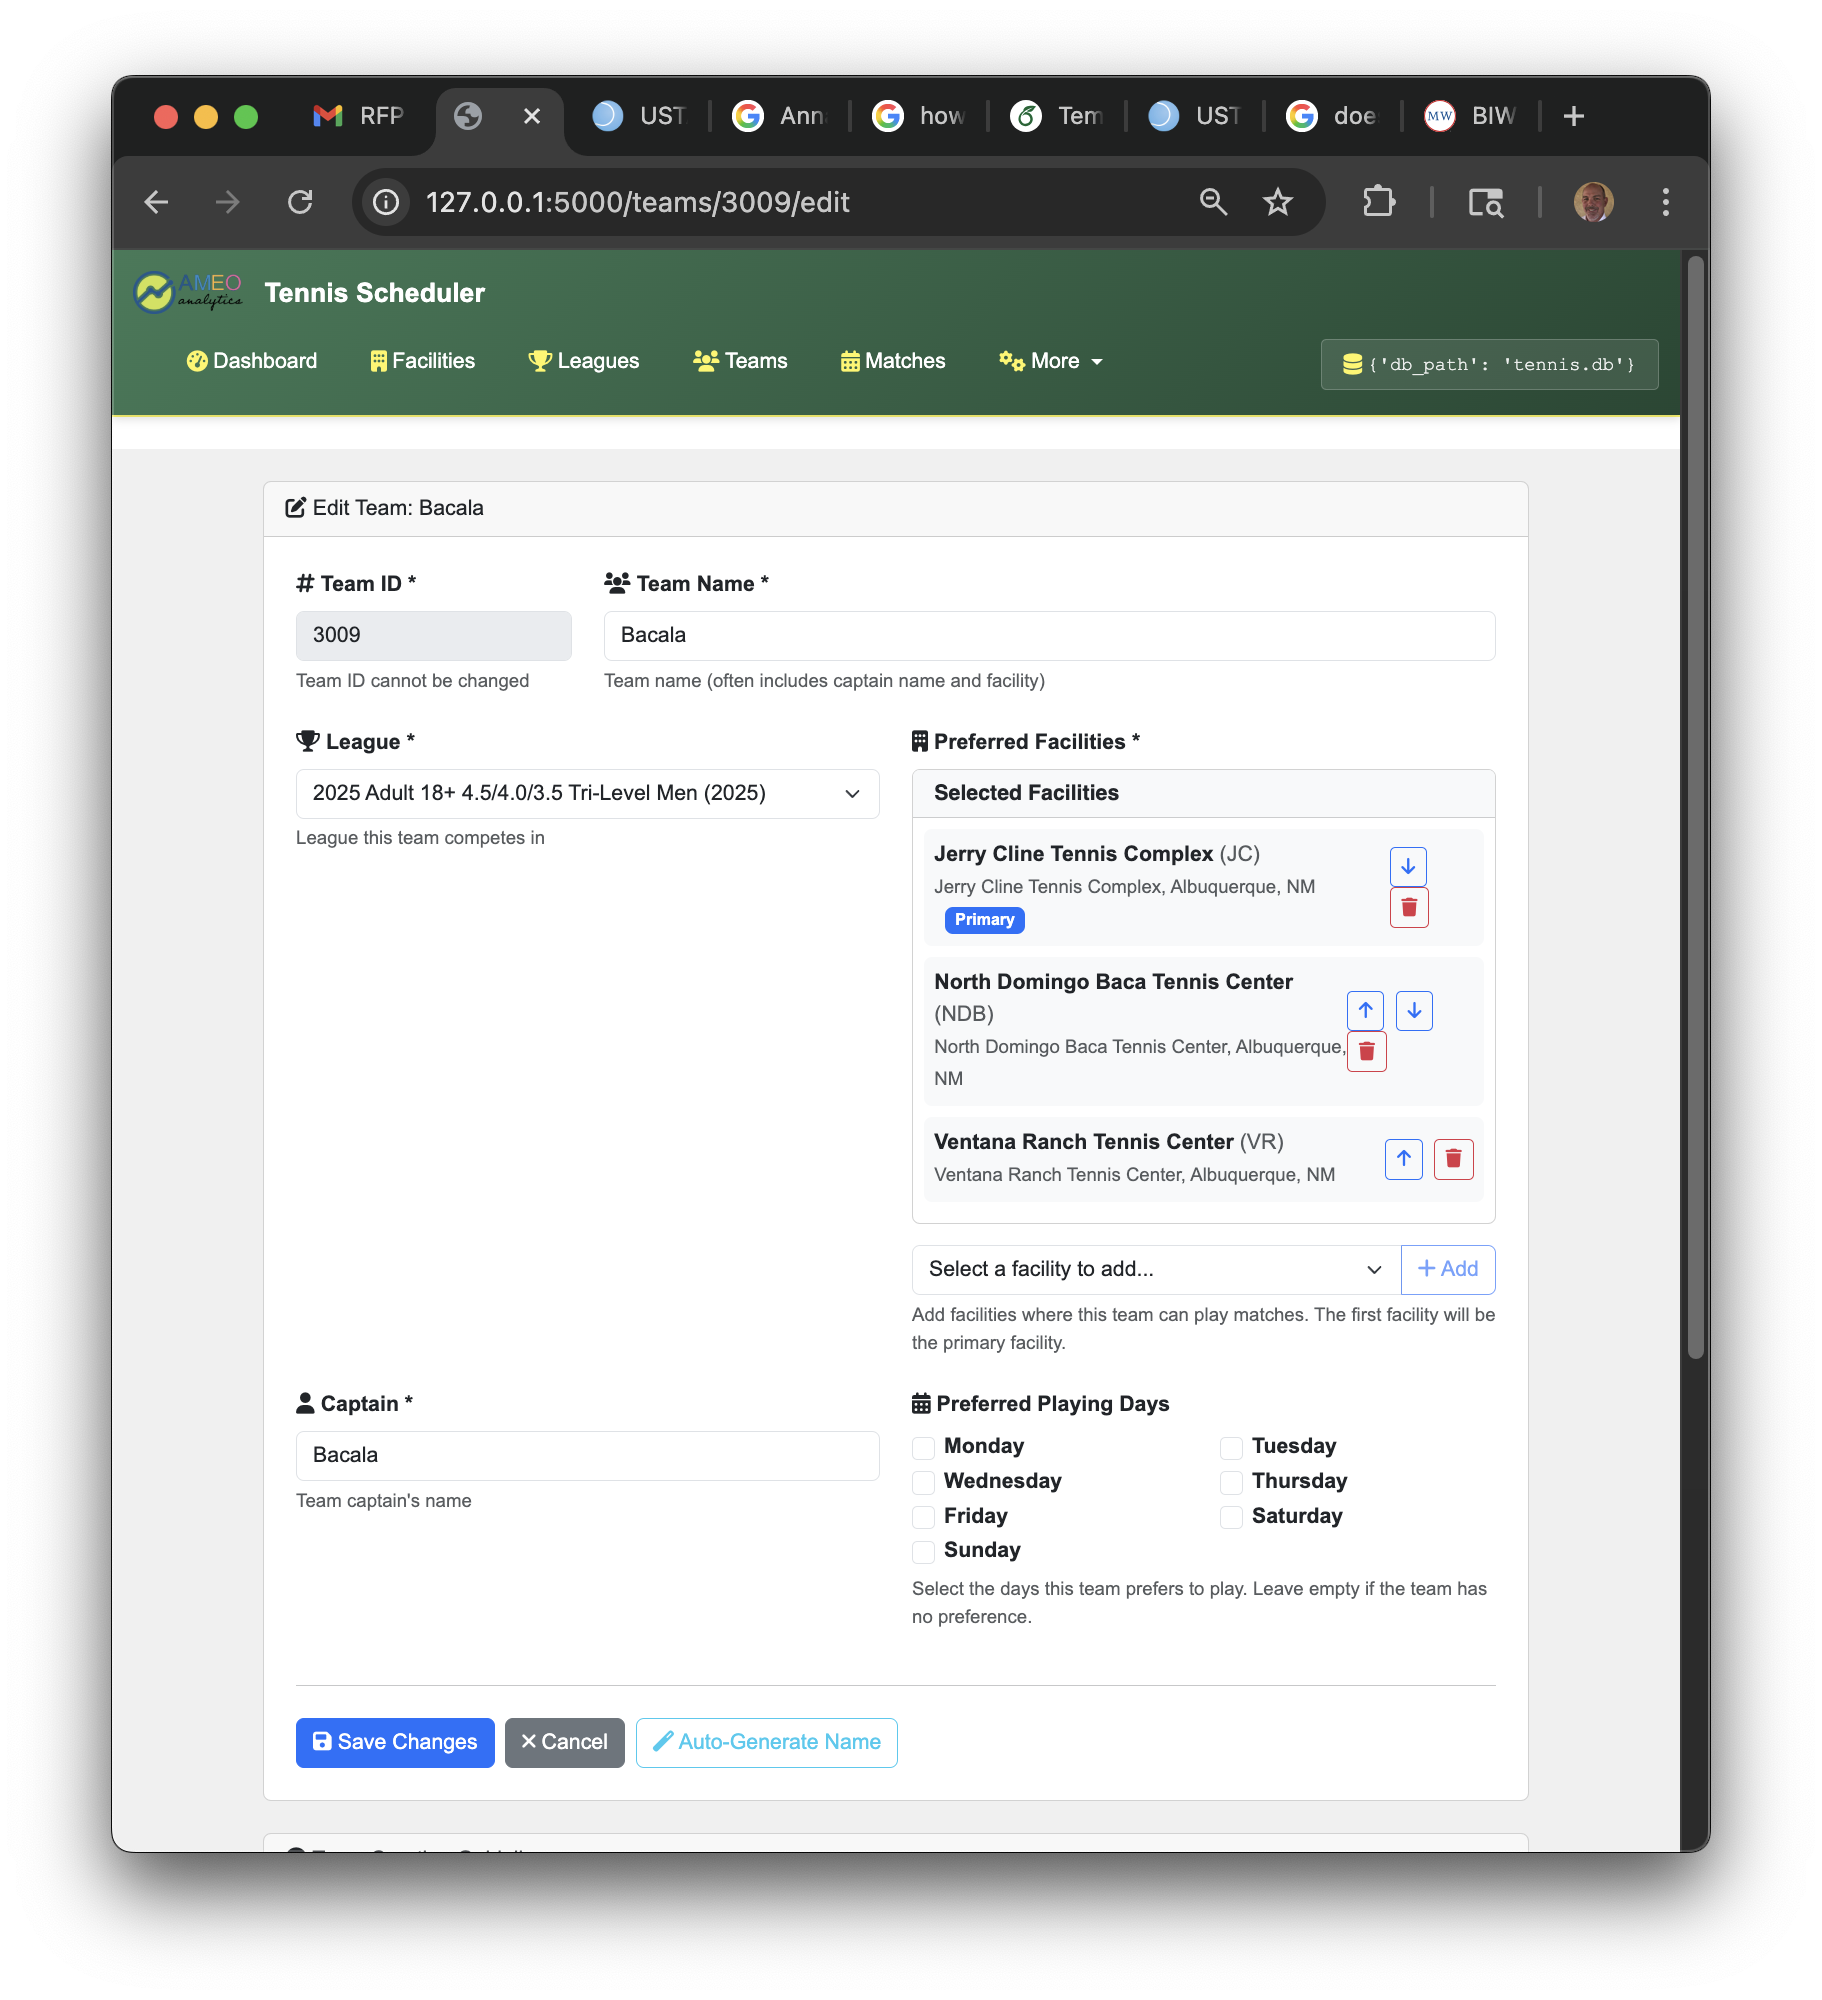
\includegraphics[width=\textwidth]{images/team-edit.png}
\end{minipage}
\caption{Team Management Interface: (left) team listing with league filtering and facility assignments, (right) team editing with multi-facility preference configuration}
\label{fig:team-management}
\end{figure}

\subsection{Advanced Match Scheduling and Optimization Framework}

\subsubsection{Automated Match Generation and Distribution}
The system implements sophisticated algorithms for fair and balanced match generation across league structures:

\begin{itemize}
    \item \textbf{Round-Robin Tournament Generation}: Implements complete round-robin algorithms ensuring every team competes against every other team exactly once per round, with balanced match distribution and equitable home/away venue assignments
    \item \textbf{Venue Equity Optimization}: Employs mathematical optimization algorithms to equalize home and away match distributions across all participating teams
    \item \textbf{Load Balancing Algorithms}: Minimizes variance in total match assignments per team to ensure competitive balance across the league structure
    \item \textbf{Configurable Tournament Structure}: Provides flexible round configuration capabilities including customizable match quantities and line specifications based on league requirements
    \item \textbf{Constraint Validation Framework}: Implements comprehensive validation systems preventing impossible scheduling scenarios through team availability analysis
\end{itemize}

\subsubsection{Intelligent Automated Scheduling Engine}
The application features a sophisticated multi-algorithm scheduling engine designed to optimize match placement:

\begin{itemize}

    \item \textbf{Team Preference Analysis}: Implements intelligent analysis algorithms for both team's preferred playing schedules and availability constraints
    \item \textbf{League Priority Hierarchies}: Considers organizational scheduling preferences including primary playing days, alternative playing days, and priorities for in-round scheduling
    \item \textbf{Real-Time Availability Processing}: Features dynamic court availability verification with integrated blackout period handling and capacity management
    \item \textbf{Conflict Resolution Protocols}: Implements comprehensive conflict detection preventing team double-booking and facility resource overbooking across all scheduling operations
    \item \textbf{Quality Assessment Metrics}: Features quantitative scoring system (0-100 scale) evaluating in-round scheduling, team, league, and facility preference alignment to assign a score to a single scheduled match
    \item \textbf{Scheduled Quality Index}: Assigns an aggregate quality score, defined as a \emph{Schedule Quality Index (SQI)} to a set of matches
    \item \textbf{Iterative Optimization Algorithms}: Employs multi-iteration scheduling with randomized seed generation to identify a schedule with the highest SQI
    \item \textbf{Adaptive Line Distribution}: Intelligent line distribution algorithms to accommodate facility capacity limitations (e.g., all lines together or split across consecutive time slots)
\end{itemize}

\subsubsection{Interactive Manual Scheduling Interface}
The system provides comprehensive manual scheduling capabilities for administrative oversight and customization:

\begin{itemize}
    \item \textbf{Visual Temporal Navigation}: Implements intuitive date browsing interface displaying quality assessment scores and comprehensive facility information
    \item \textbf{Dynamic Conflict Visualization}: Real-time display of existing match conflicts, court availability status, and potential scheduling conflicts
    \item \textbf{Multi-Modal Scheduling Options}: Flexible scheduling methodologies including:
    \begin{itemize}
        \item All lines together: All match lines scheduled simultaneously
        \item Split lines: Match lines split across multiple time slots
        \item Custom scheduling: Individual line scheduling providing maximum administrative flexibility (TODO)
    \end{itemize}
    \item \textbf{Transaction Preview Capabilities}: Comprehensive preview functionality displaying all proposed database modifications prior to commitment
    \item \textbf{Validation and Warning Systems}: Advanced warning mechanisms identifying scheduling conflicts and suboptimal administrative choices
\end{itemize}

\begin{figure}[htbp]
\centering
\begin{minipage}{0.48\textwidth}
\centering
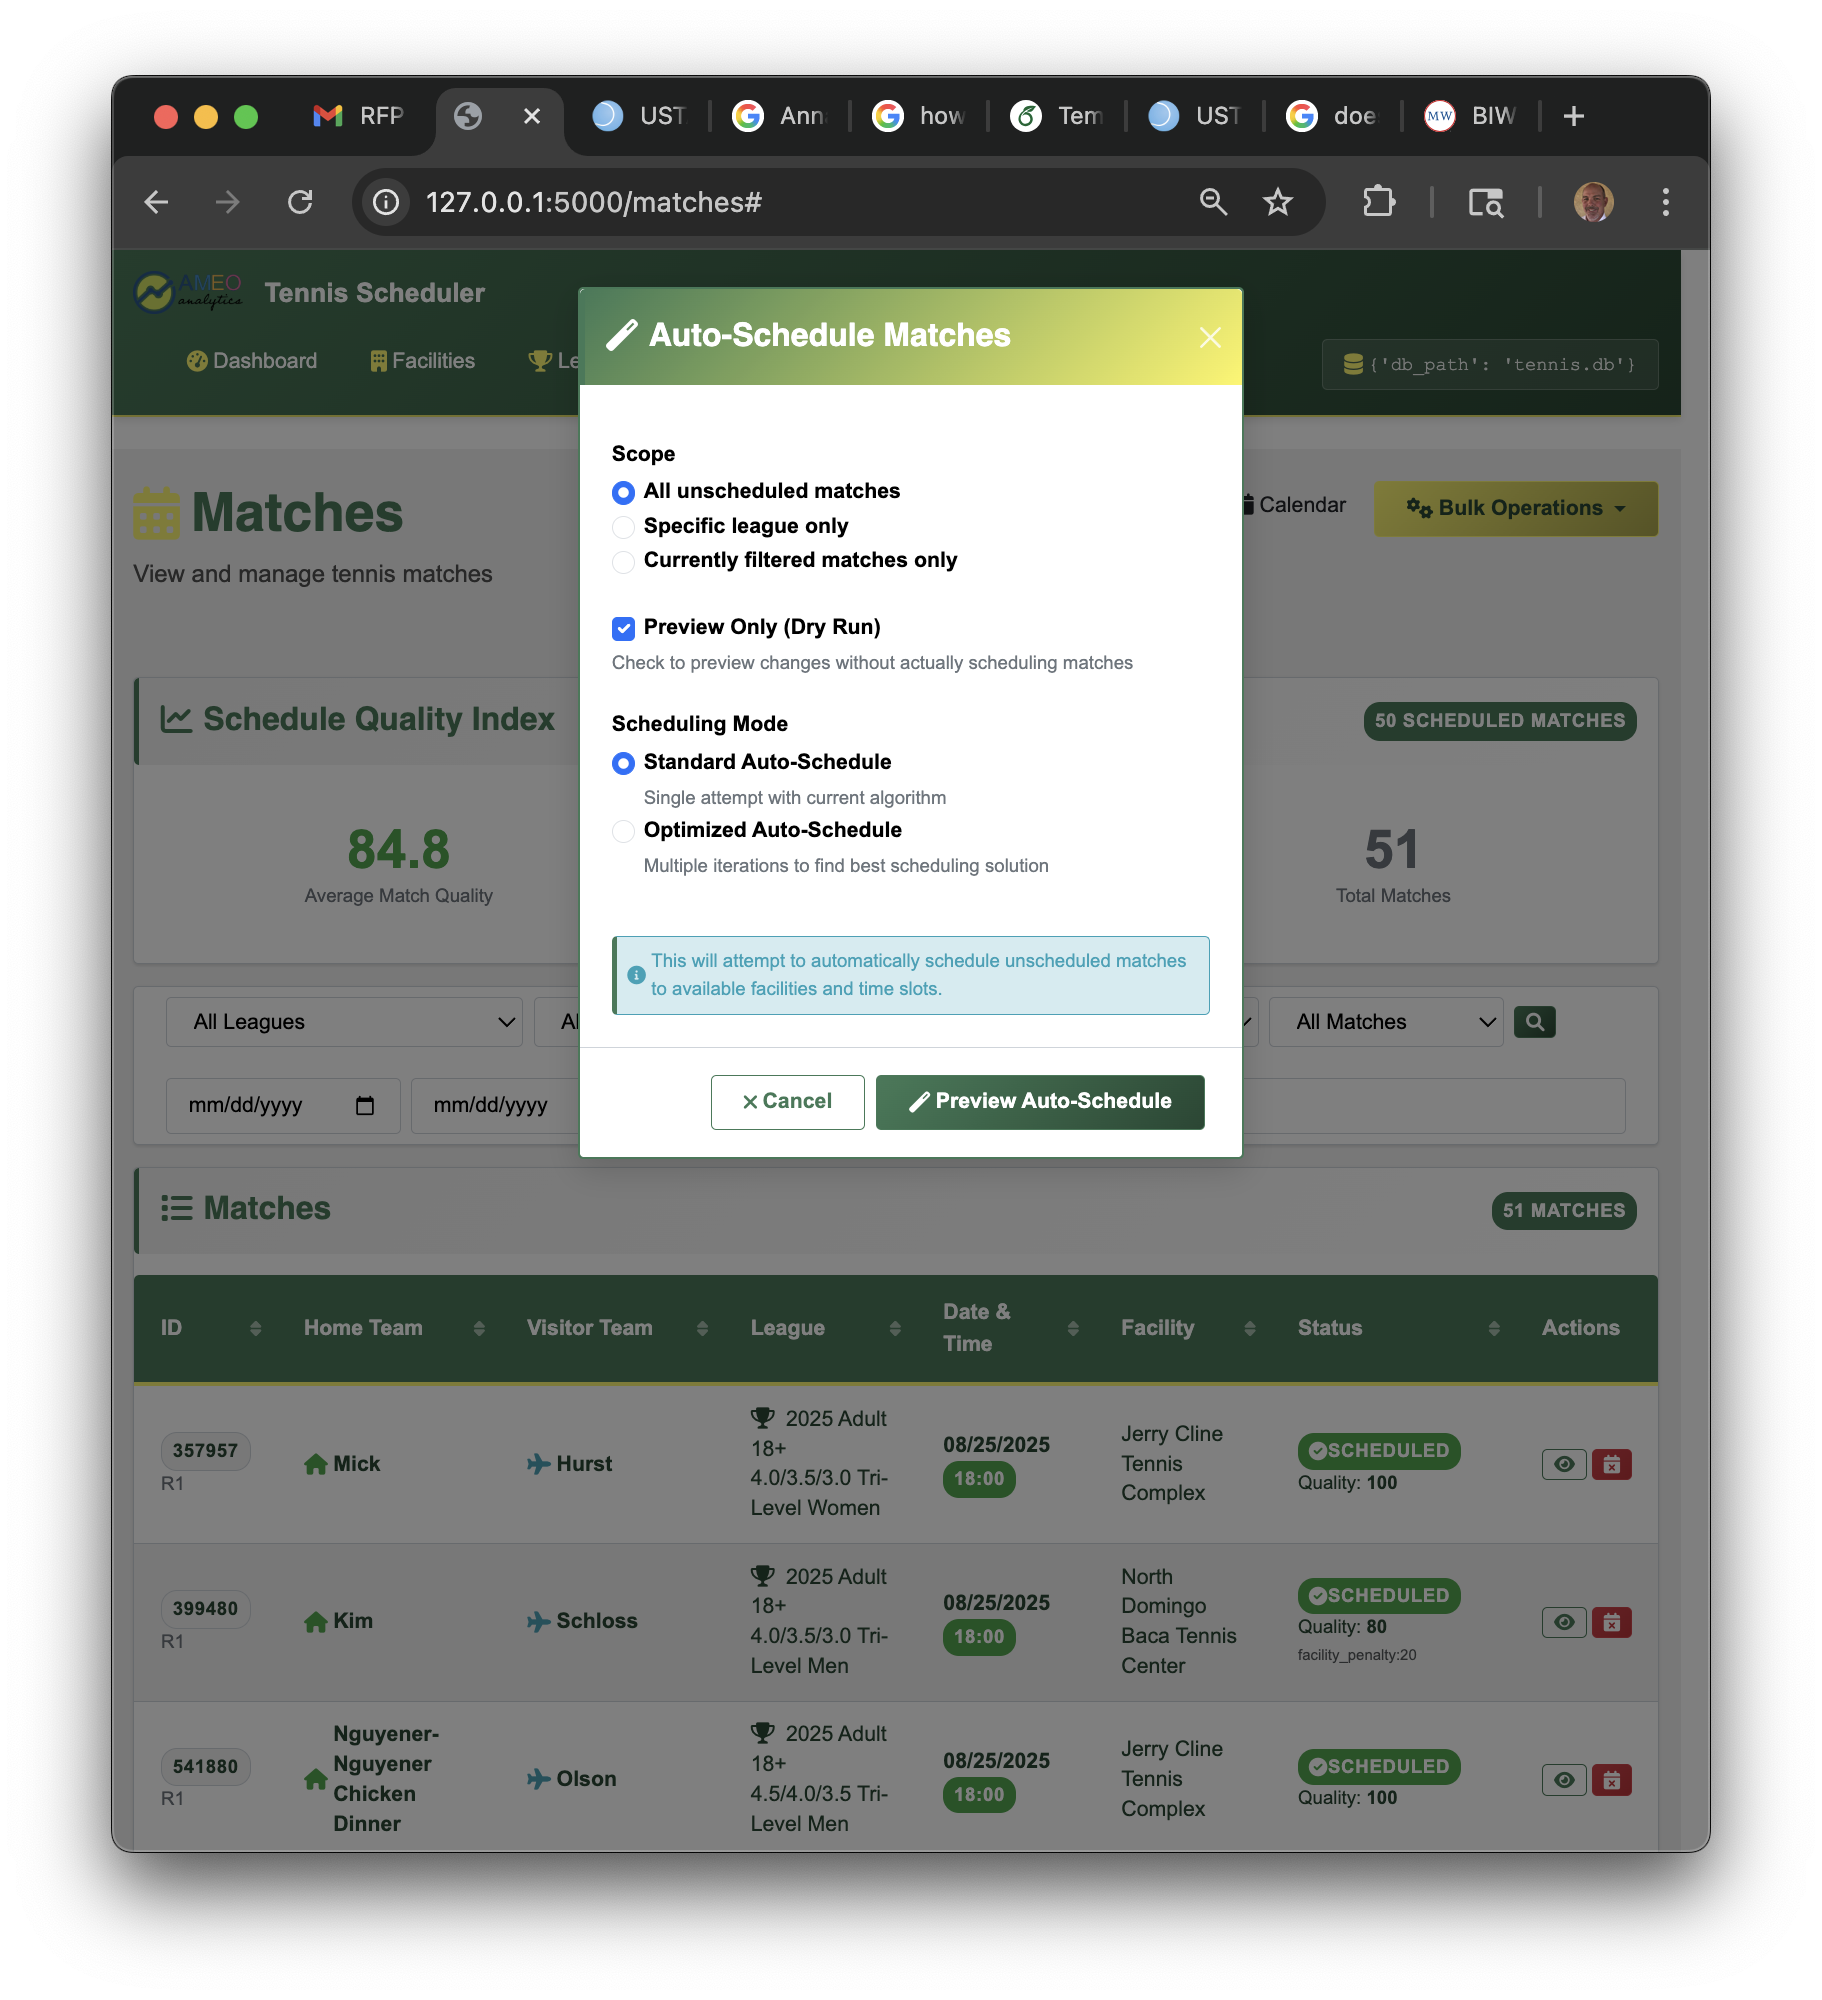
\includegraphics[width=\textwidth]{images/matches-schedule.png}
\end{minipage}
\hfill
\begin{minipage}{0.48\textwidth}
\centering
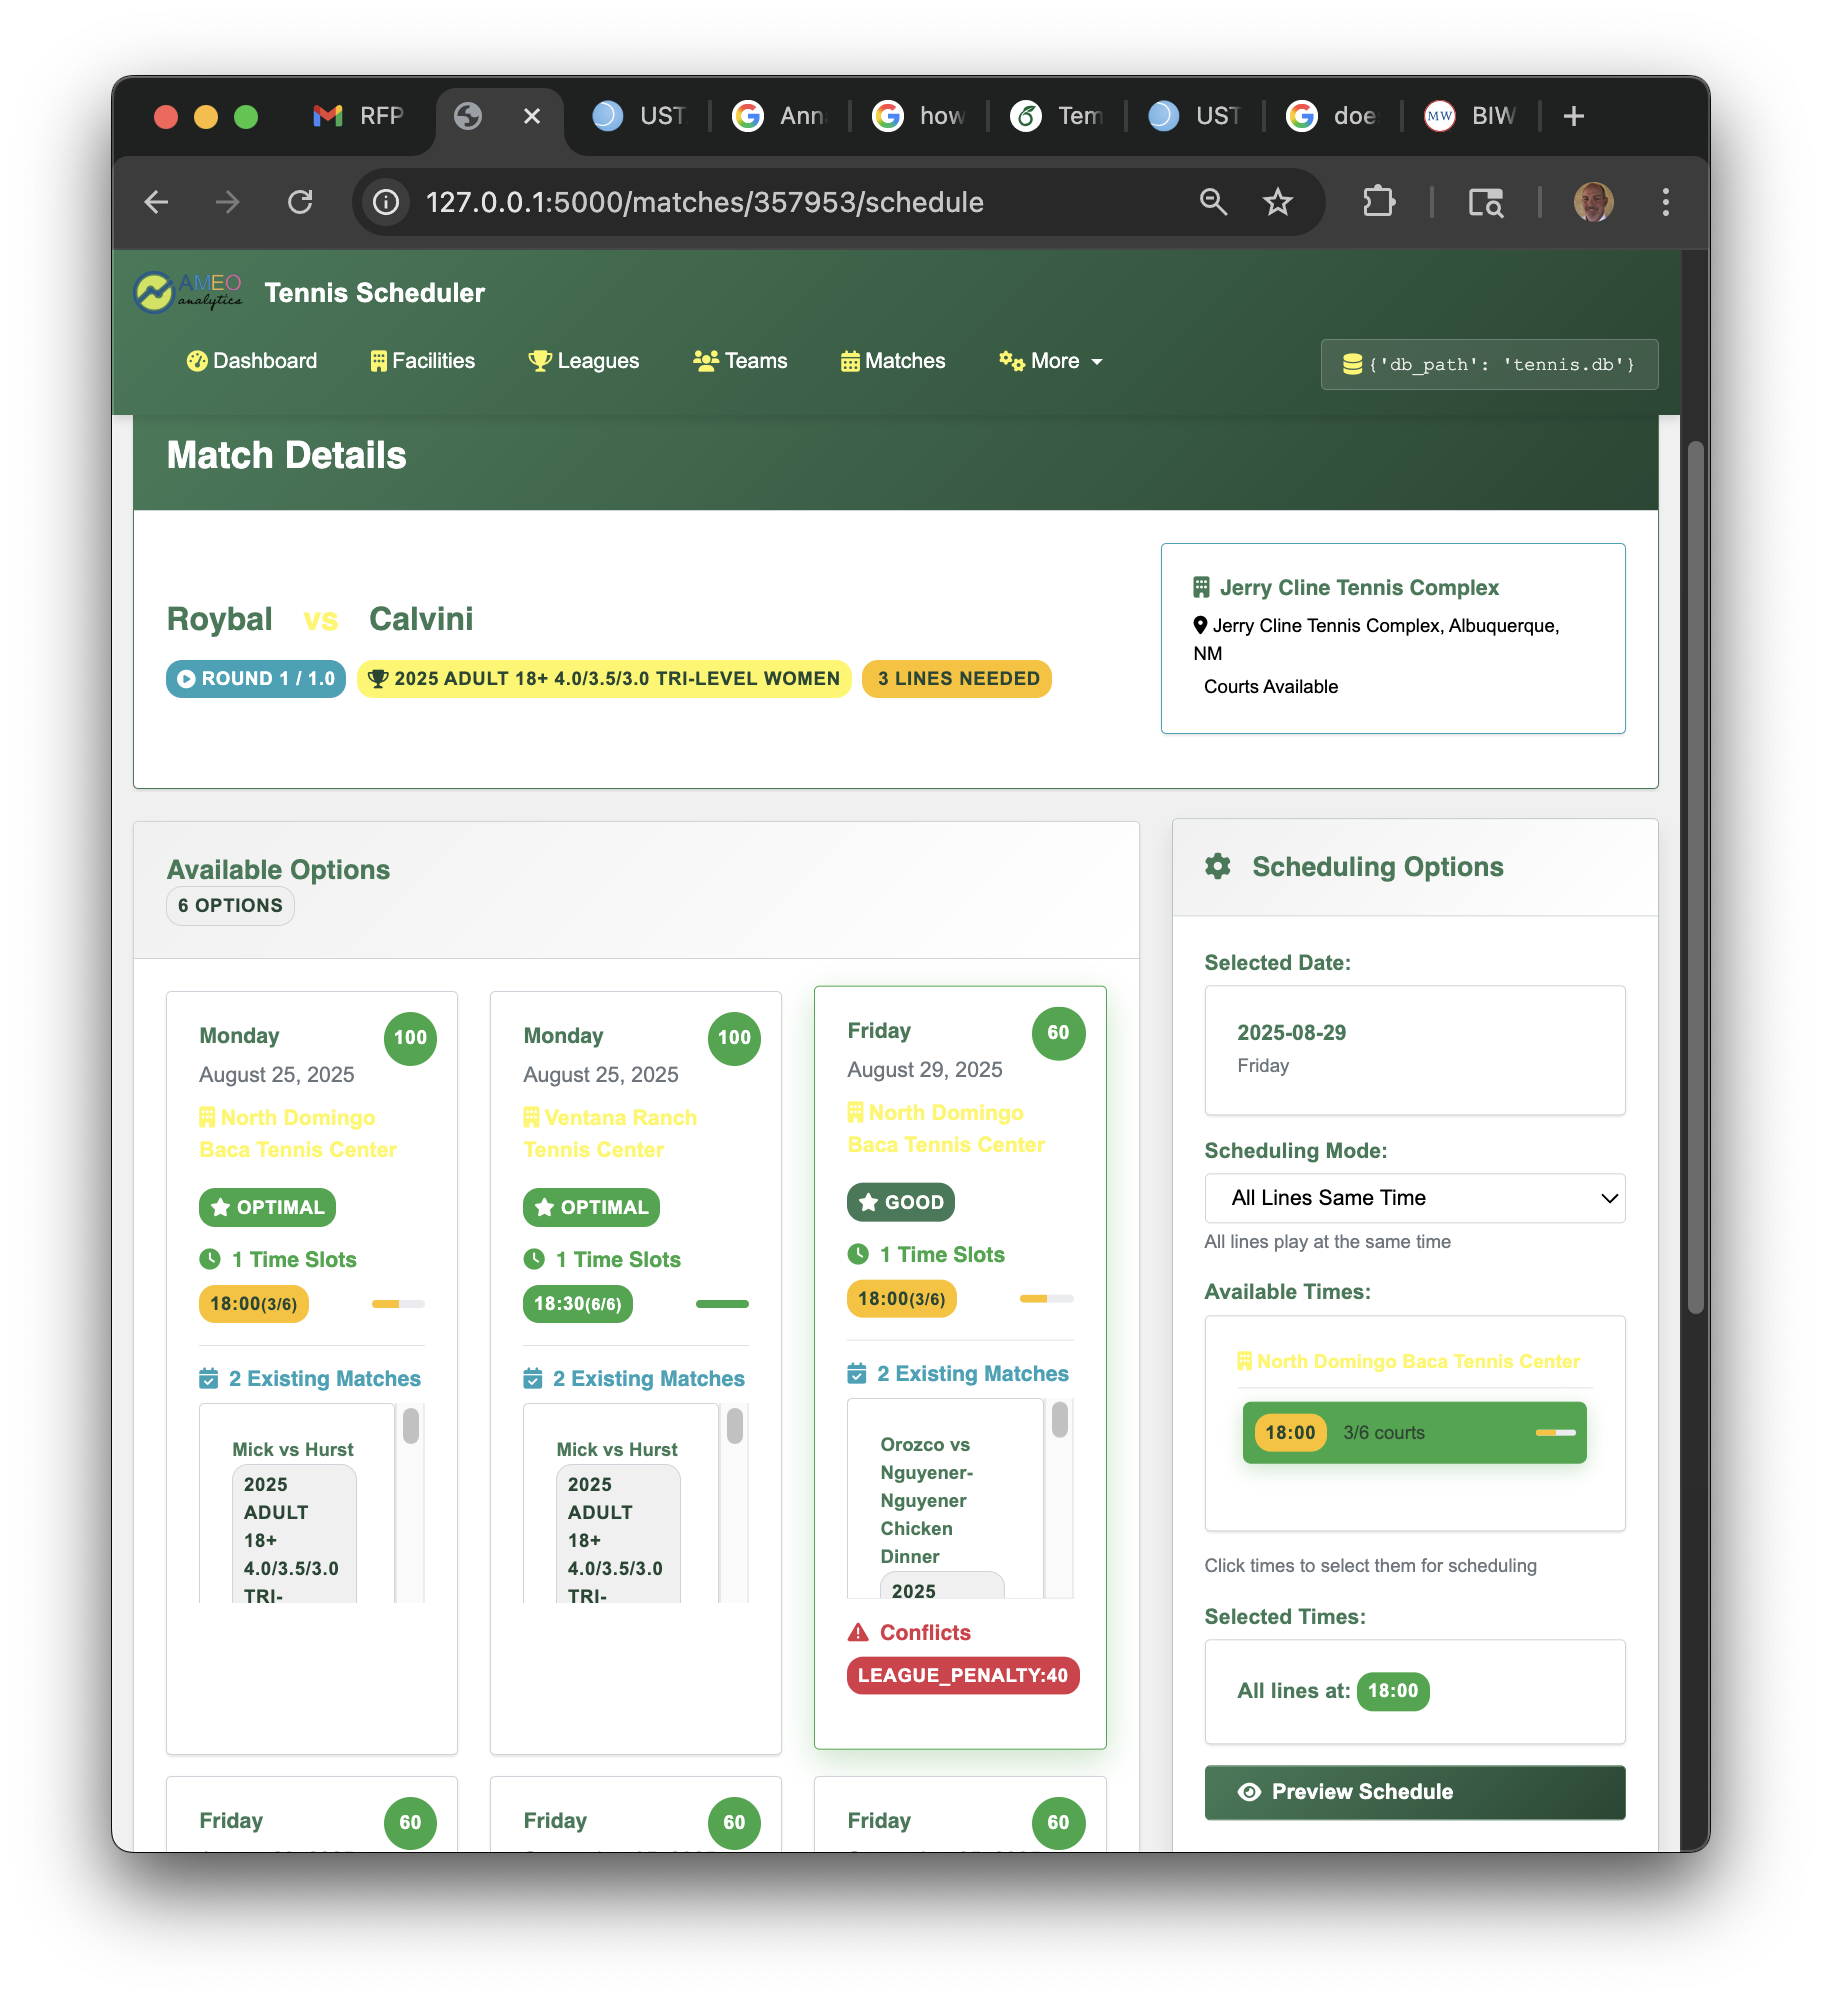
\includegraphics[width=\textwidth]{images/match-schedule.png}
\end{minipage}
\caption{Scheduling Interfaces: (left) match listing with scheduling controls and quality assessment highlighing the bulk match-scheduling capability, (right) individual match scheduling showing options and with quality scores.}
\label{fig:manual-scheduling}
\end{figure}

% \subsubsection{Advanced Optimization and Performance Analytics}
% The application implements sophisticated optimization and analytical capabilities:

% \begin{itemize}
%     \item \textbf{Multi-Iteration Optimization Framework}: Executes multiple automated scheduling attempts utilizing diverse randomization seeds (configurable 1-100 iterations)
%     \item \textbf{Performance Metrics Analysis}: Comprehensive quality metrics tracking across optimization iterations to identify optimal scheduling configurations
%     \item \textbf{Bulk Operation Management}: Advanced bulk processing capabilities including automated match scheduling with preview functionality, bulk unscheduling, and deletion operations
%     \item \textbf{Transaction Safety Protocols}: Comprehensive dry-run capabilities with transaction rollback functionality for failed operations
%     \item \textbf{Temporal Visualization Tools}: Interactive calendar interfaces providing monthly and weekly views of scheduled match distributions
% \end{itemize}

\begin{figure}[htbp]
\centering
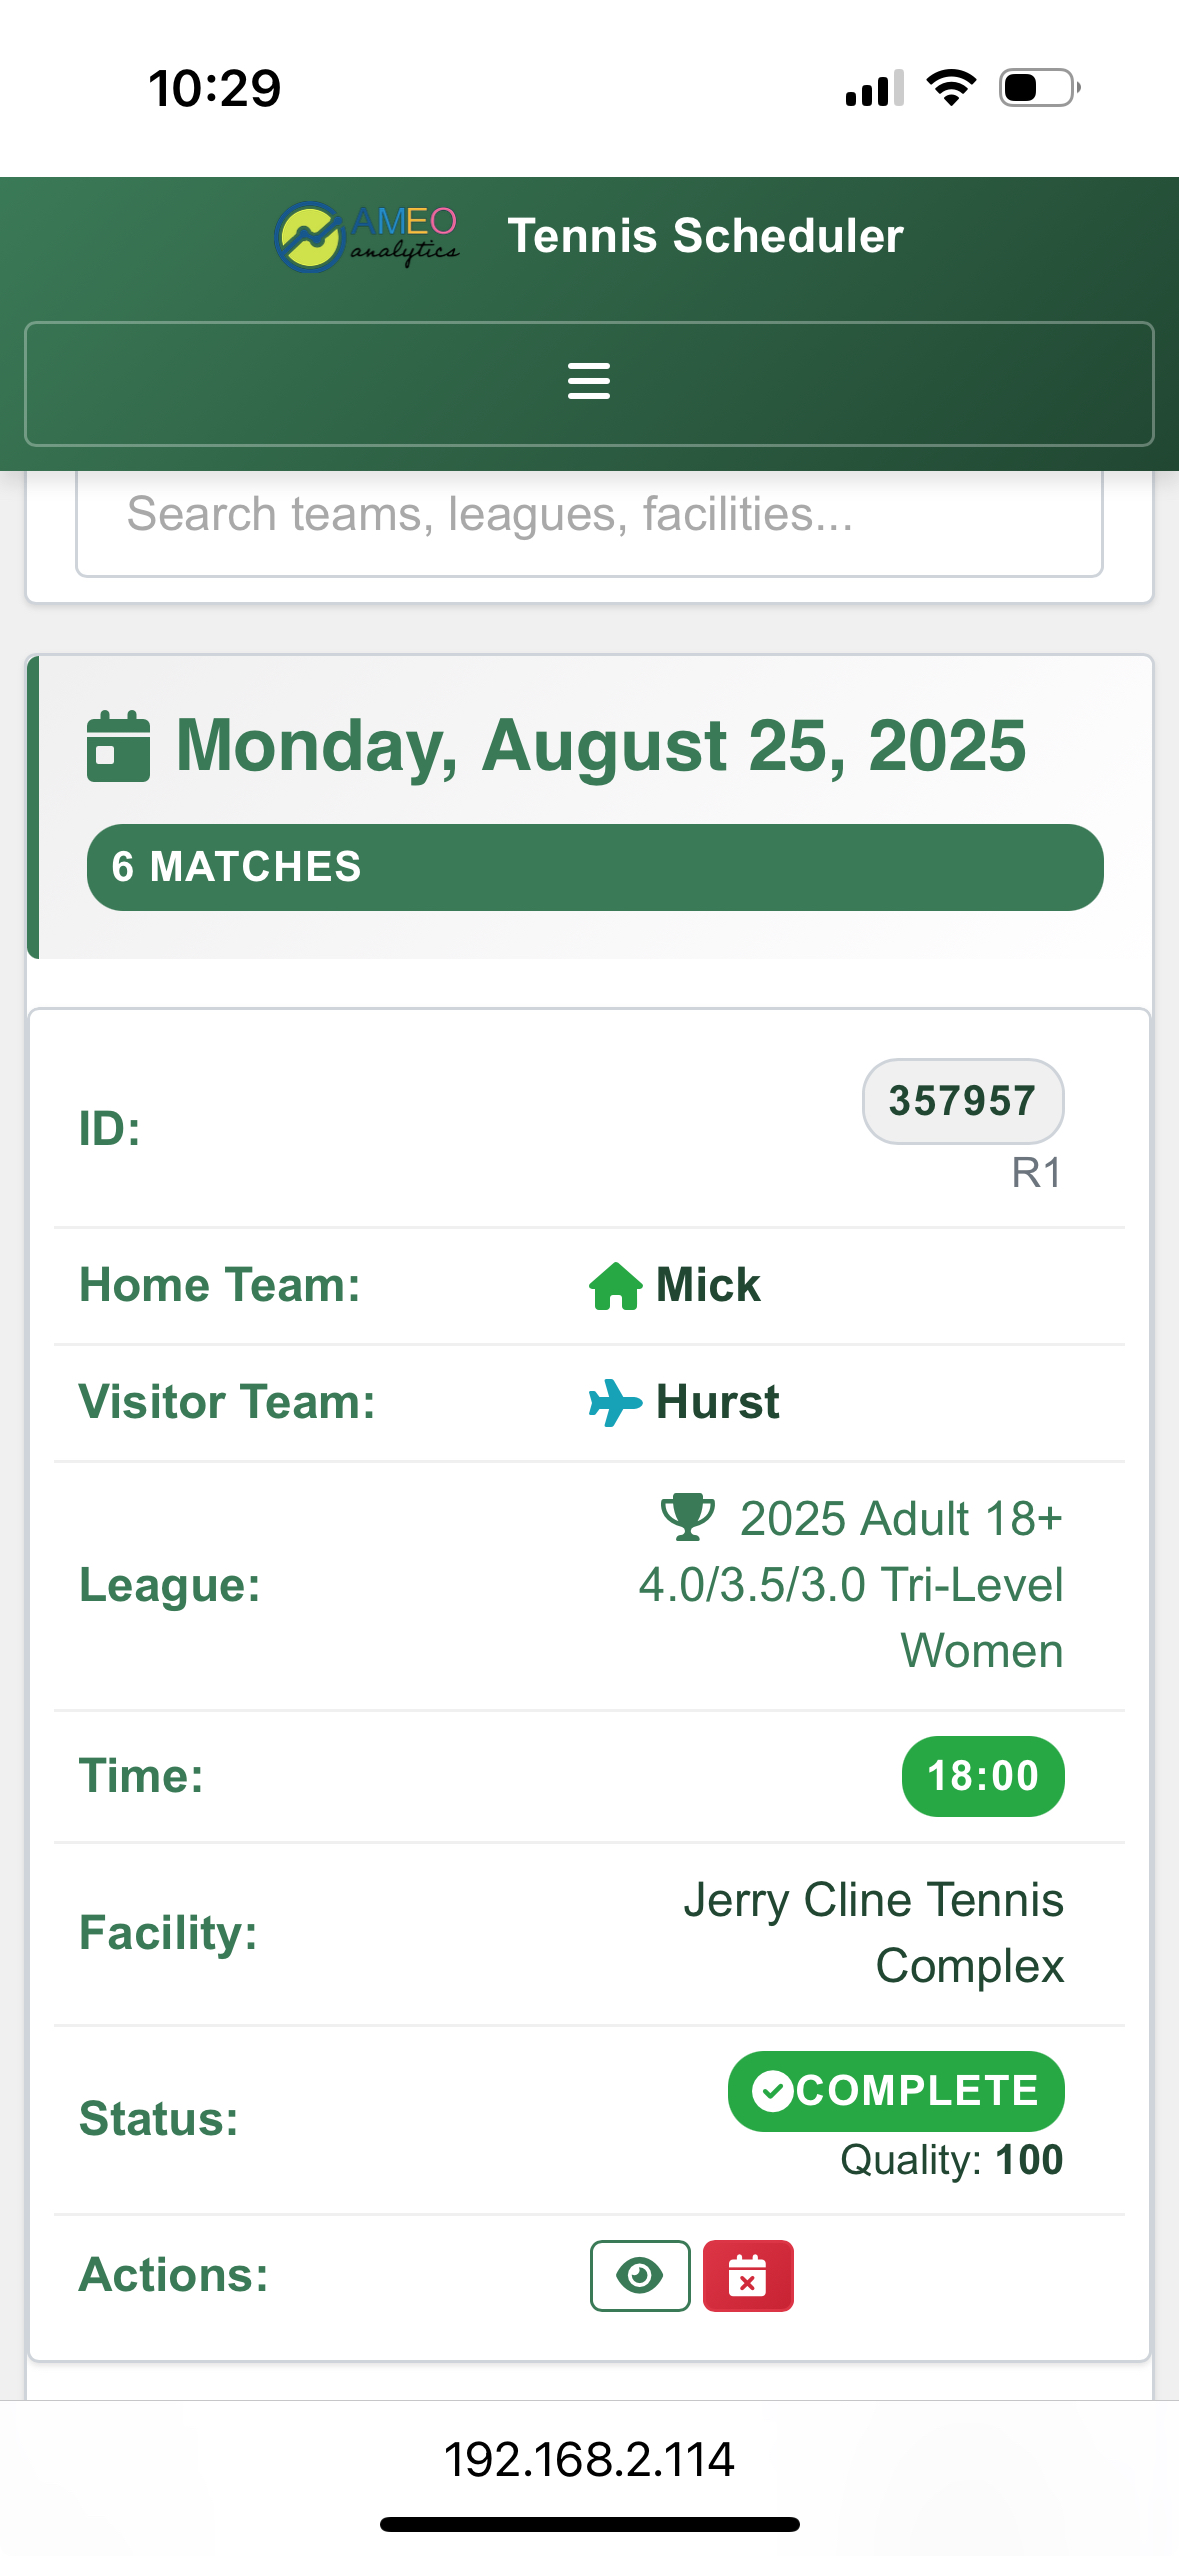
\includegraphics[width=0.3\textwidth]{images/matches-cell.jpg}
\caption{Mobile-phone interface for scheduled matches.}
\label{fig:calendar-view}
\end{figure}

\subsection{Data Integration and Management Framework}

\subsubsection{Advanced Import/Export Architecture}
The system implements comprehensive data interchange capabilities supporting multiple formats and complex data structures:

\begin{itemize}
    \item \textbf{Multi-Format Data Interchange}: Comprehensive import and export functionality supporting both YAML and JSON formats for leagues, facilities, teams, and match data structures
    \item \textbf{Composite Data File Support}: Advanced capability supporting heterogeneous data files containing any combination of organizational entities (leagues, facilities, teams, matches) within single import/export operations
    \item \textbf{Intelligent Content Processing}: Automated content detection and processing algorithms with comprehensive error handling protocols and real-time progress tracking mechanisms
    \item \textbf{Data Integrity Validation}: Robust YAML-based data validation framework with comprehensive integrity checking and bulk operation support
\end{itemize}

\subsubsection{Administrative Command Line Interface}
The application provides a comprehensive command-line interface for administrative operations, system automation, and feature testing:

\begin{itemize}
    \item \textbf{Safe Operation Protocols}: All administrative operations default to preview mode with explicit execution flags required for system modifications
    \item \textbf{Operation Transparency}: Comprehensive preview functionality providing detailed operation descriptions prior to execution
    \item \textbf{Transaction Integrity}: Full ACID compliance implementation ensuring complete data integrity across all operations
    \item \textbf{Integrated Testing Framework}: Built-in comprehensive testing capabilities accessible through command-line interface with extensive test suite coverage
\end{itemize}

\subsection{Supplementary Capabilities and Enhancement Features}

The application includes additional value-added features that enhance operational efficiency and user experience:

\begin{itemize}
    \item \textbf{USTA Reference Integration}: Comprehensive reference database of official USTA organizational structures including sections, regions, age groups, and divisions for accurate league configuration
    \item \textbf{Statistical Analysis Dashboard}: Advanced analytical capabilities providing database overviews, entity counts, and detailed league breakdowns with comprehensive team and match analytics
    \item \textbf{Cross-Platform Compatibility}: Bootstrap-based responsive design architecture ensuring optimal functionality across mobile and desktop platforms
    \item \textbf{Advanced Analytics and Reporting}: Sophisticated facility utilization analytics and scheduling quality metrics with performance optimization insights
    \item \textbf{Type Safety Framework}: Strict mypy configuration with comprehensive type hint implementation ensuring code reliability and maintainability
\end{itemize}



\subsection{Technical Architecture and Implementation Framework}

The system employs sophisticated software engineering principles and architectural patterns:

\begin{itemize}
    \item \textbf{Modular Interface Architecture}: Implementation of pluggable database backend systems through comprehensive TennisDBInterface abstraction layers
    \item \textbf{Specialized Database Implementation}: Full-featured SQLite backend with specialized entity management systems for optimal performance
    \item \textbf{Factory Design Pattern}: TennisDBFactory implementation for systematic database instance creation and lifecycle management
    \item \textbf{Domain-Specific Entity Management}: Specialized management modules for leagues, teams, facilities, matches, and scheduling operations

\end{itemize}

